\documentclass[runningheads]{llncs}

% ---------------------------------------------------------------
% Include basic ECCV package
 
% TODO REVIEW: Insert your submission number below by replacing '*****'
% TODO FINAL: Comment out the following line for the camera-ready version
\usepackage[review,year=2024,ID=7833]{eccv}
% TODO FINAL: Un-comment the following line for the camera-ready version
%\usepackage{eccv}

% OPTIONAL: Un-comment the following line for a version which is easier to read
% on small portrait-orientation screens (e.g., mobile phones, or beside other windows)
%\usepackage[mobile]{eccv}


% ---------------------------------------------------------------
% Other packages

% Commonly used abbreviations (\eg, \ie, \etc, \cf, \etal, etc.)
\usepackage{eccvabbrv}

% Include other packages here, before hyperref.
\usepackage{graphicx}
\usepackage{booktabs}
\usepackage{listings}
\usepackage{multirow}

% The "axessiblity" package can be found at: https://ctan.org/pkg/axessibility?lang=en
\usepackage[accsupp]{axessibility}  % Improves PDF readability for those with disabilities.


% ---------------------------------------------------------------
% Hyperref package

% It is strongly recommended to use hyperref, especially for the review version.
% Please disable hyperref *only* if you encounter grave issues.
% hyperref with option pagebackref eases the reviewers' job, but should be disabled for the final version.
%
% If you comment hyperref and then uncomment it, you should delete
% main.aux before re-running LaTeX.
% (Or just hit 'q' on the first LaTeX run, let it finish, and you
%  should be clear).

% TODO FINAL: Comment out the following line for the camera-ready version
\usepackage[pagebackref,breaklinks,colorlinks,citecolor=eccvblue]{hyperref}
% TODO FINAL: Un-comment the following line for the camera-ready version
%\usepackage{hyperref}

% Support for ORCID icon
\usepackage{orcidlink}

\newcommand{\todo}[1]{\textcolor{red}{TODO: #1}\PackageWarning{TODO:}{#1!}}
% ---------------------------------------------------------------
% structured language syntax highlighting
\lstdefinestyle{dtypestyle}{ basicstyle=\ttfamily\bfseries\color{blue} }
\lstdefinestyle{cmdstyle}{ basicstyle=\ttfamily\bfseries\color{black} }
\newcommand{\paramstyle}[2]{{\textbf{\texttt{\textcolor{#1}{#2}}}}}


% Define custom language
\definecolor{darkgray}{gray}{0.3}
\definecolor{darkgreen}{RGB}{50, 150, 50}
\definecolor{darkred}{RGB}{180, 50, 50}
\definecolor{darkblue}{RGB}{80, 106, 156}
\definecolor{col1}{HTML}{506A88}
\definecolor{col2}{HTML}{2E3D47}
\definecolor{col3}{HTML}{98A9B5}
\definecolor{col4}{HTML}{D19C83}
\definecolor{fom}{RGB}{0,153,139}

\lstdefinelanguage{StructuredLanguage}
{
  basicstyle=\ttfamily\bfseries,
  morekeywords={id, a_x, a_b, a_z, b_x, b_y, b_z, position_x, position_y, position_z, wall0_id, wall1_id, width, height, thickness, wall_id, pos_x, pos_y, size_x, size_y},
  keywords = [2]{string, bool, int, float},
  keywords = [3]{make_wall, make_wall_prim, make_door, make_bbox, make_prim,make_curved_wall},
  keywordstyle=\color{darkgray},
  keywordstyle=[2]\bfseries\color{blue},
  keywordstyle=[3]\bfseries\color{blue},
  sensitive=false,
  breaklines=true
}

% Define style for different types of tokens
\lstset{language=StructuredLanguage}

\begin{document}
\newcommand{\techTerm}[1]{\emph{#1}}
\newcommand{\Aria}{\techTerm{Aria}}
\newcommand{\AStar}{\techTerm{A*}}
\newcommand{\Blender}{\techTerm{Blender}}
\newcommand{\CGAL}{\techTerm{CGAL}}
\newcommand{\COLMAP}{\techTerm{COLMAP}}
\newcommand{\Euston}{\techTerm{METHODNAME}}
\newcommand{\GeometryNodes}{\techTerm{geometry nodes}}
\newcommand{\GLB}{\techTerm{GLB}}
\newcommand{\IMU}{\techTerm{IMU}}
\newcommand{\LLM}{\techTerm{LLM}}
\newcommand{\LSDSLAM}{\techTerm{LSD-SLAM}}
\newcommand{\PyBullet}{\techTerm{PyBullet}}
\newcommand{\RGB}{\techTerm{RGB}}
\newcommand{\SLAM}{\techTerm{SLAM}}
\newcommand{\SfM}{\techTerm{SfM}}
\newcommand{\Trimesh}{\techTerm{Trimesh}}


% method names etc
\newcommand{\METHOD}{\texttt{SceneScript}}
\newcommand{\DatasetName}{\techTerm{Aria Synthetic Environments}}
% \newcommand{\DatasetName}{\techTerm{Anonymized Dataset}}
\newcommand{\DatasetNameShort}{\techTerm{ASE}}
% \newcommand{\DatasetNameShort}{\techTerm{Anon. Dataset}}


\definecolor{table_bbox_color}{rgb}{0.788, 0.742, 0.657}
\definecolor{sofa_bbox_color}{rgb}{0.152, 0.328, 0.536}
\definecolor{shelf_bbox_color}{rgb}{0.371, 0.524, 0.487}
\definecolor{chair_bbox_color}{rgb}{0.349, 0.573, 0.460}
\definecolor{bed_bbox_color}{rgb}{0.800, 0.680, 0.858}
\definecolor{floor_mat_bbox_color}{rgb}{0.364, 0.028, 0.243}
\definecolor{exercise_weight_bbox_color}{rgb}{0.417, 0.190, 0.343}
\definecolor{cutlery_bbox_color}{rgb}{0.599, 0.360, 0.998}
\definecolor{container_bbox_color}{rgb}{0.572, 0.788, 0.191}
\definecolor{clock_bbox_color}{rgb}{0.185, 0.021, 0.629}
\definecolor{cart_bbox_color}{rgb}{0.557, 0.555, 0.620}
\definecolor{vase_bbox_color}{rgb}{0.784, 0.853, 0.415}
\definecolor{tent_bbox_color}{rgb}{0.942, 0.780, 0.475}
\definecolor{flower_pot_bbox_color}{rgb}{0.555, 0.602, 0.953}
\definecolor{pillow_bbox_color}{rgb}{0.167, 0.193, 0.815}
\definecolor{mount_bbox_color}{rgb}{0.885, 0.425, 0.074}
\definecolor{lamp_bbox_color}{rgb}{0.360, 0.078, 0.494}
\definecolor{ladder_bbox_color}{rgb}{0.309, 0.204, 0.255}
\definecolor{fan_bbox_color}{rgb}{0.853, 0.804, 0.618}
\definecolor{cabinet_bbox_color}{rgb}{0.945, 0.184, 0.371}
\definecolor{jar_bbox_color}{rgb}{0.061, 0.831, 0.701}
\definecolor{picture_frame_bbox_color}{rgb}{0.623, 0.224, 0.610}
\definecolor{mirror_bbox_color}{rgb}{0.558, 0.264, 0.332}
\definecolor{electronic_device_bbox_color}{rgb}{0.534, 0.739, 0.043}
\definecolor{dresser_bbox_color}{rgb}{0.709, 0.031, 0.301}
\definecolor{clothes_rack_bbox_color}{rgb}{0.536, 0.392, 0.088}
\definecolor{battery_charger_bbox_color}{rgb}{0.043, 0.991, 0.131}
\definecolor{air_conditioner_bbox_color}{rgb}{0.241, 0.007, 0.729}
\definecolor{window_bbox_color}{rgb}{0.207, 0.942, 0.897}
% ---------------------------------------------------------------
% TODO REVIEW: Replace with your title
\title{\METHOD: Supplementary Material}

% TODO REVIEW: If the paper title is too long for the running head, you can set
% an abbreviated paper title here. If not, comment out.
\titlerunning{SceneScript}

% TODO FINAL: Replace with your author list. 
% Include the authors' OCRID for the camera-ready version, if at all possible.
\author{First Author\inst{1}\orcidlink{0000-1111-2222-3333} \and
Second Author\inst{2,3}\orcidlink{1111-2222-3333-4444} \and
Third Author\inst{3}\orcidlink{2222--3333-4444-5555}}

% TODO FINAL: Replace with an abbreviated list of authors.
\authorrunning{F.~Author et al.}
% First names are abbreviated in the running head.
% If there are more than two authors, 'et al.' is used.

% TODO FINAL: Replace with your institution list.
\institute{Princeton University, Princeton NJ 08544, USA \and
Springer Heidelberg, Tiergartenstr.~17, 69121 Heidelberg, Germany
\email{lncs@springer.com}\\
\url{http://www.springer.com/gp/computer-science/lncs} \and
ABC Institute, Rupert-Karls-University Heidelberg, Heidelberg, Germany\\
\email{\{abc,lncs\}@uni-heidelberg.de}}

\maketitle


%\clearpage
%\setcounter{page}{1}
% \maketitlesupplementary
\appendix

\section{\DatasetName{}}
\label{sec:input_data}

\begin{figure*}[ht]
    \centering
    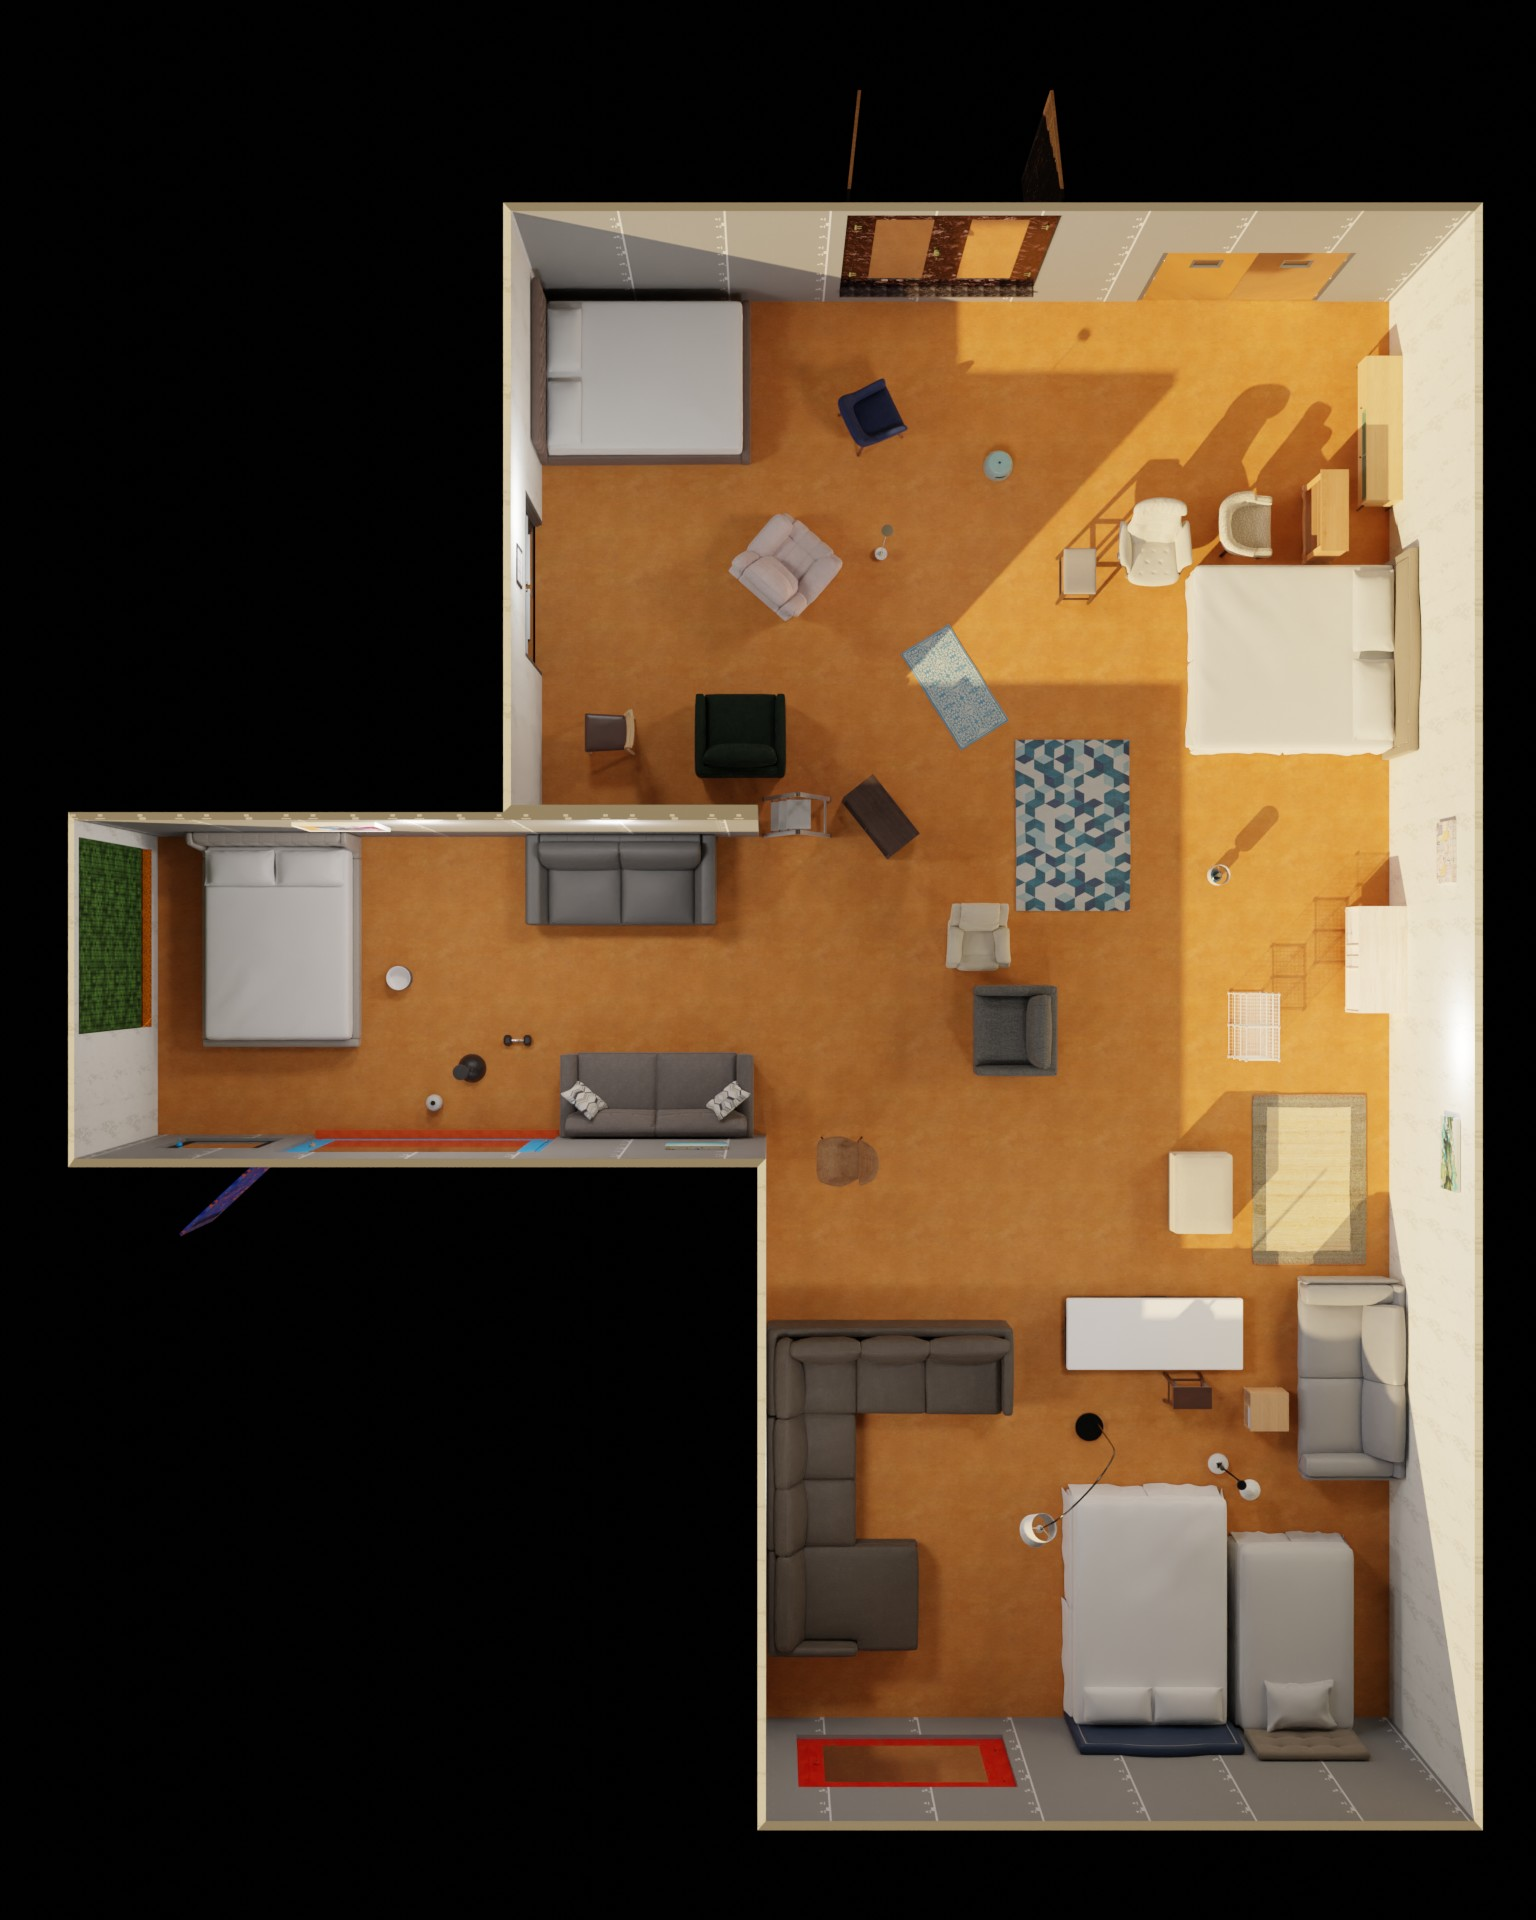
\includegraphics[width=0.24\linewidth]{figs/ase_bev_renderings/scene10.jpg} 
    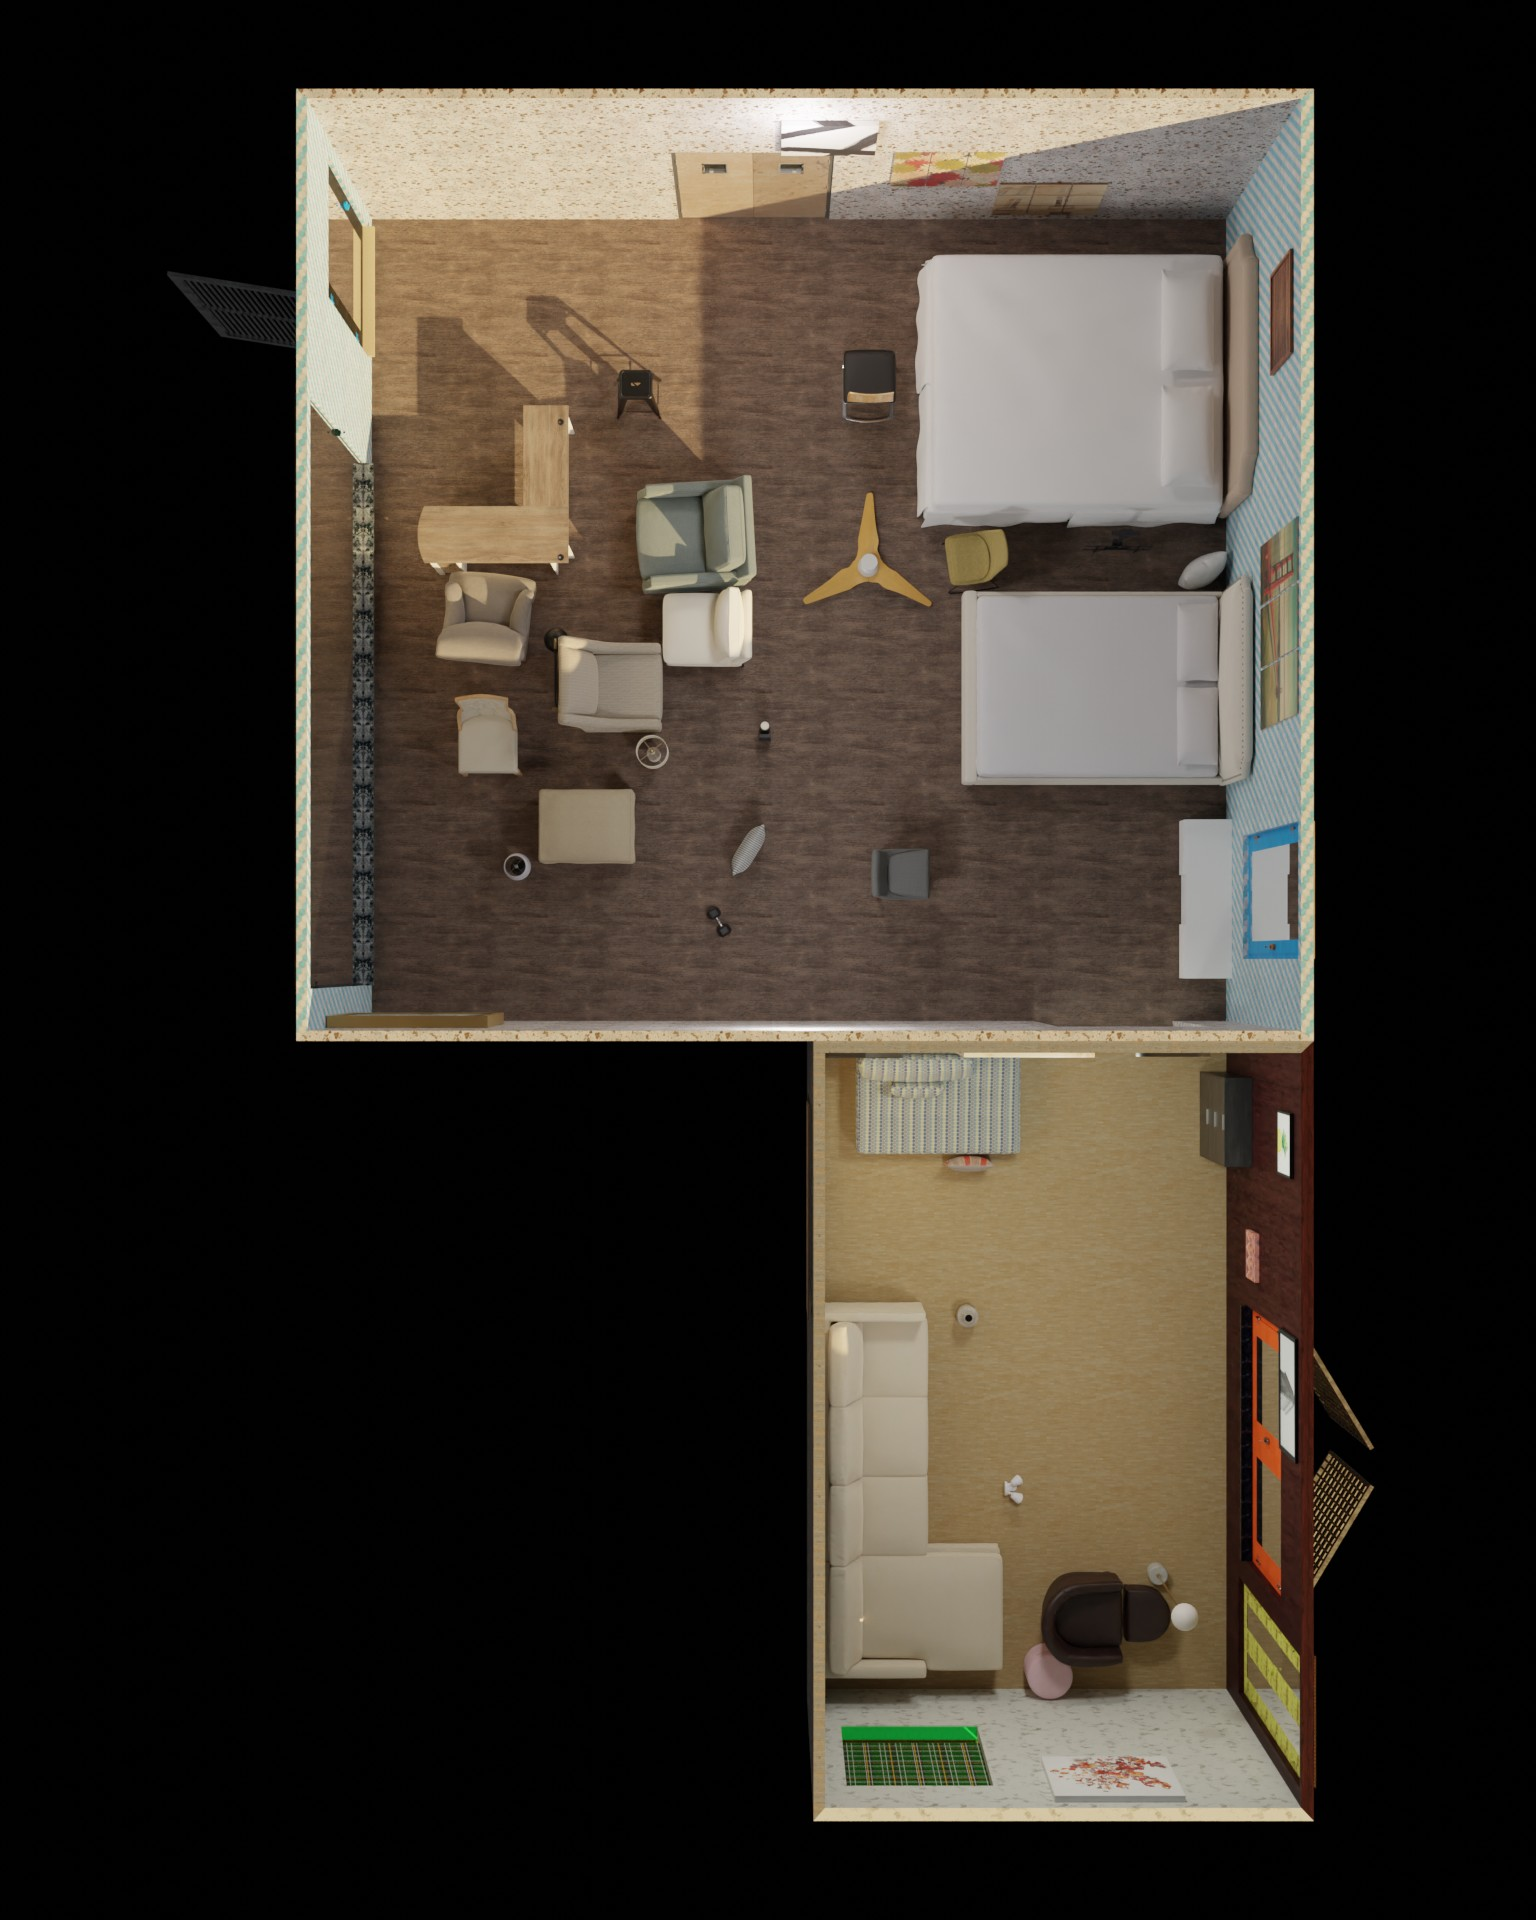
\includegraphics[width=0.24\linewidth]{figs/ase_bev_renderings/scene1024.jpg} 
    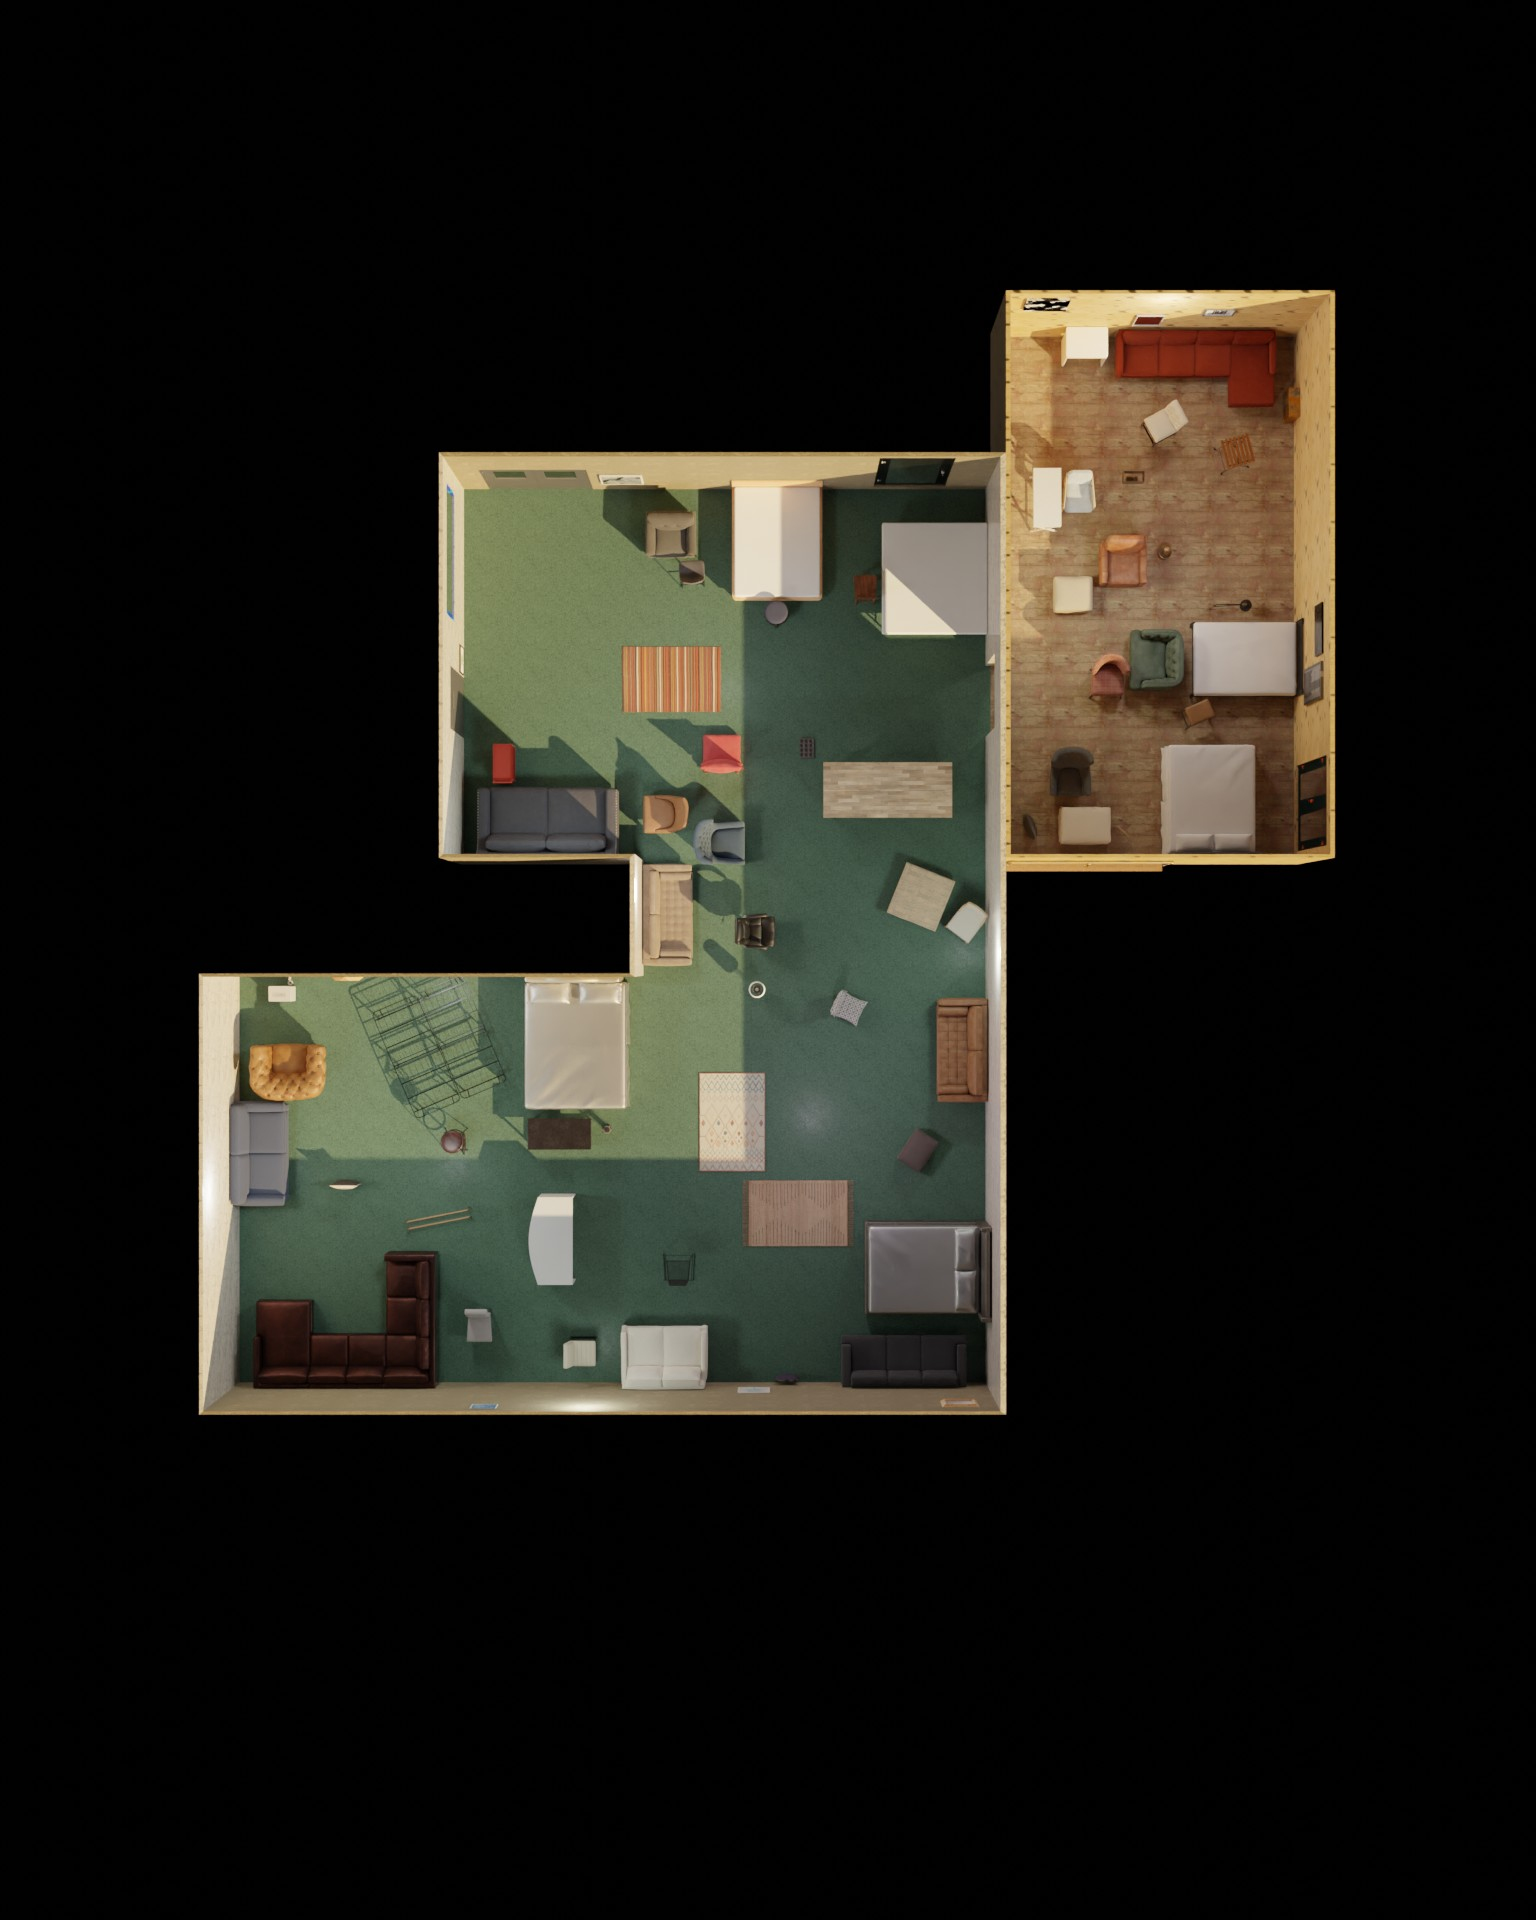
\includegraphics[width=0.24\linewidth]{figs/ase_bev_renderings/scene1029.jpg} 
    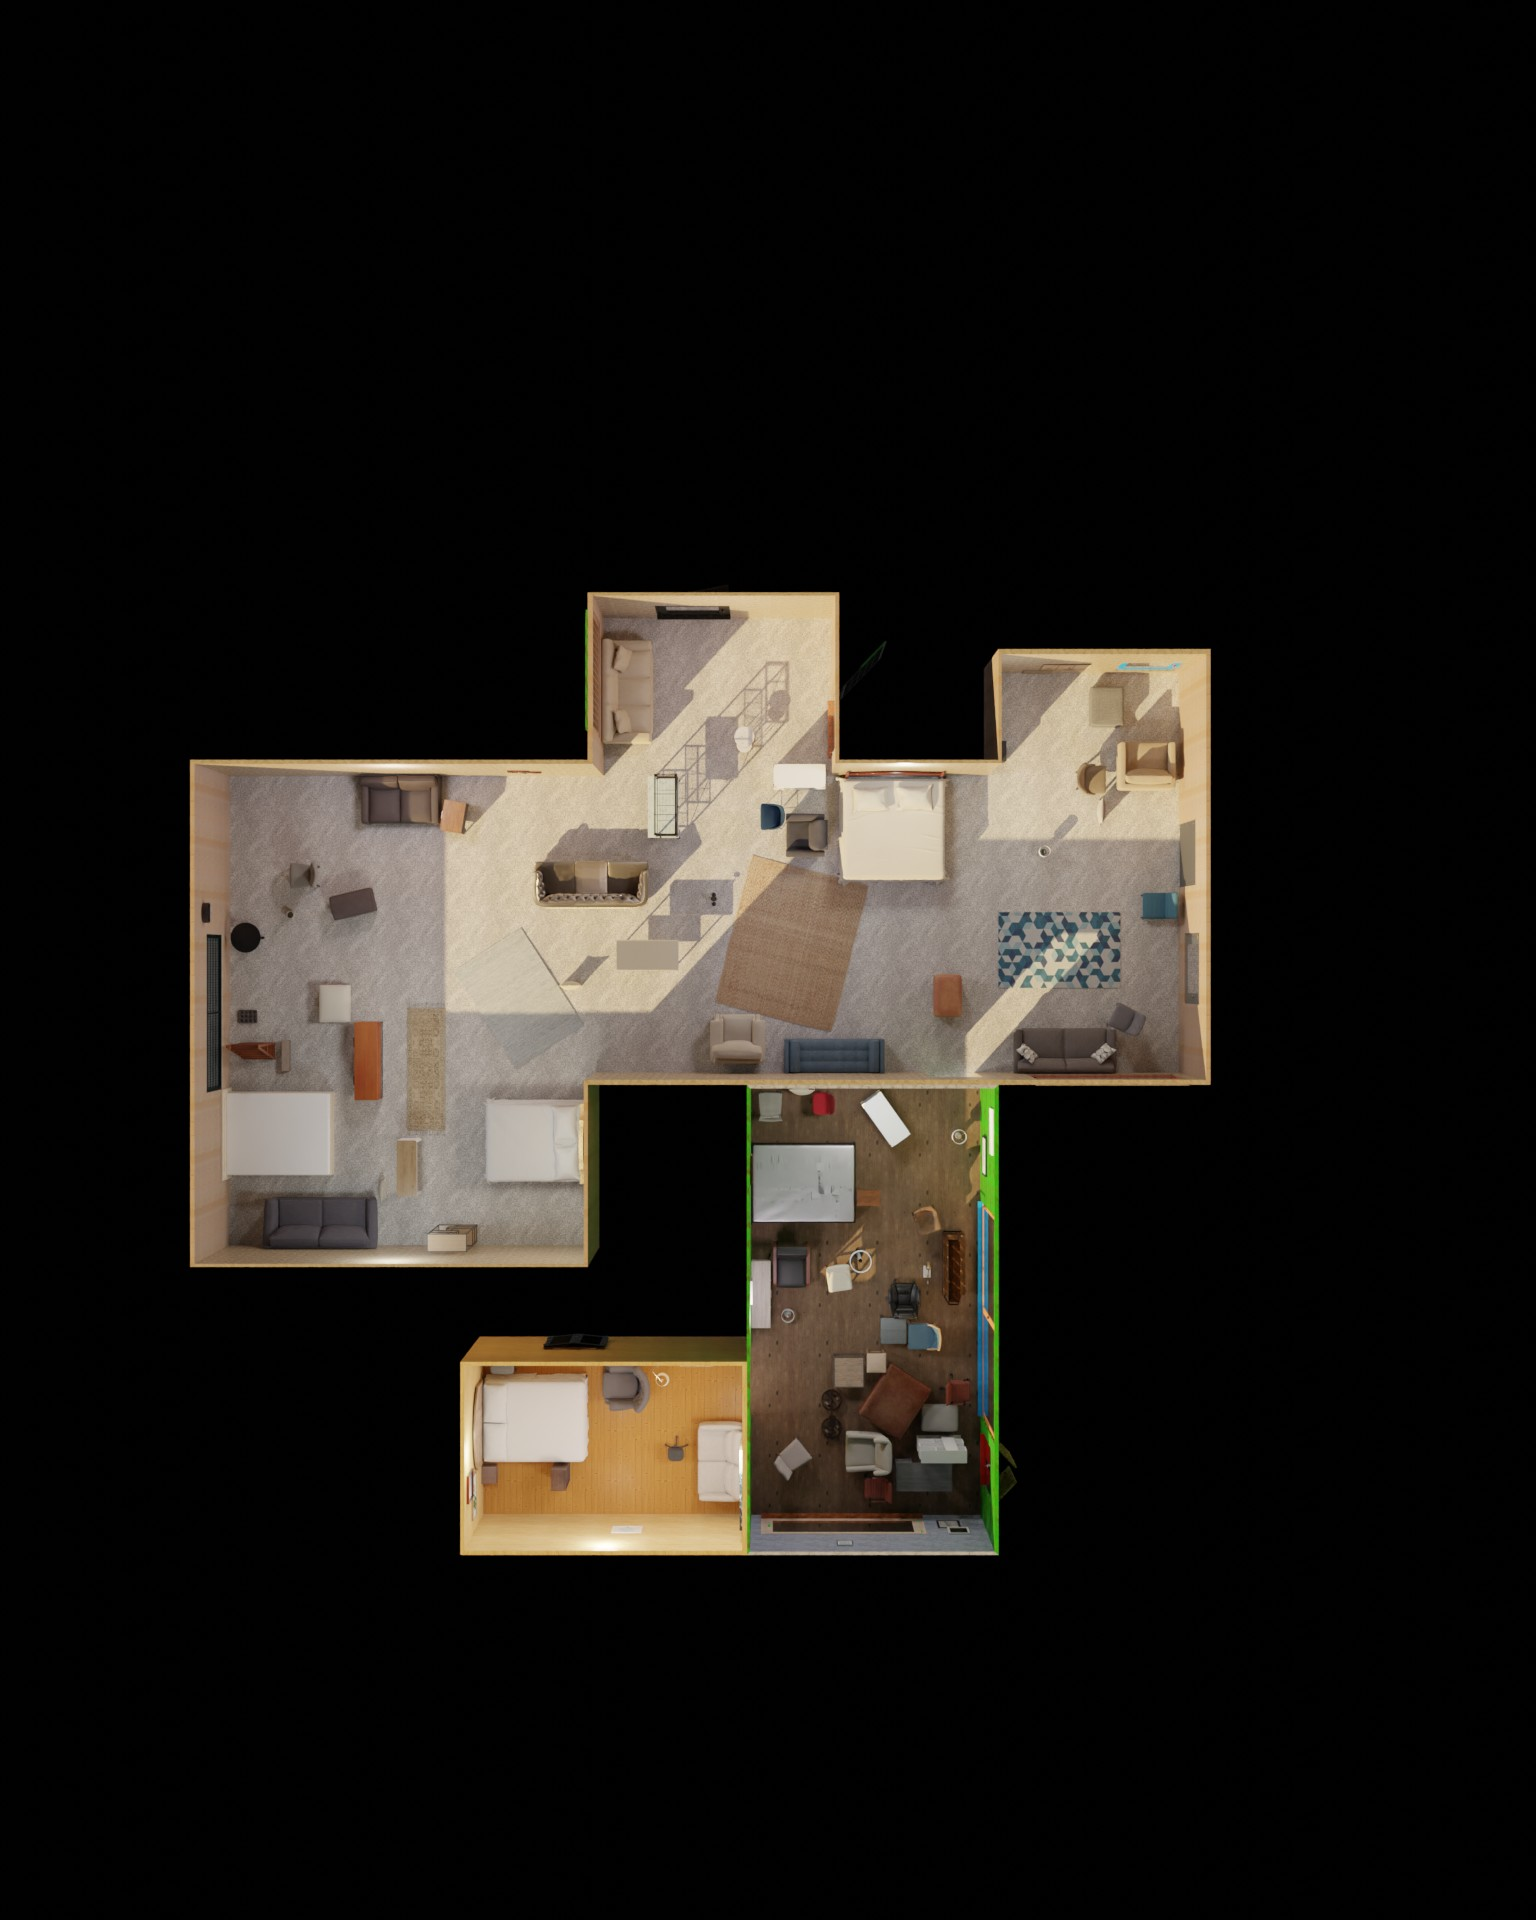
\includegraphics[width=0.24\linewidth]{figs/ase_bev_renderings/scene1437.jpg}
    %
    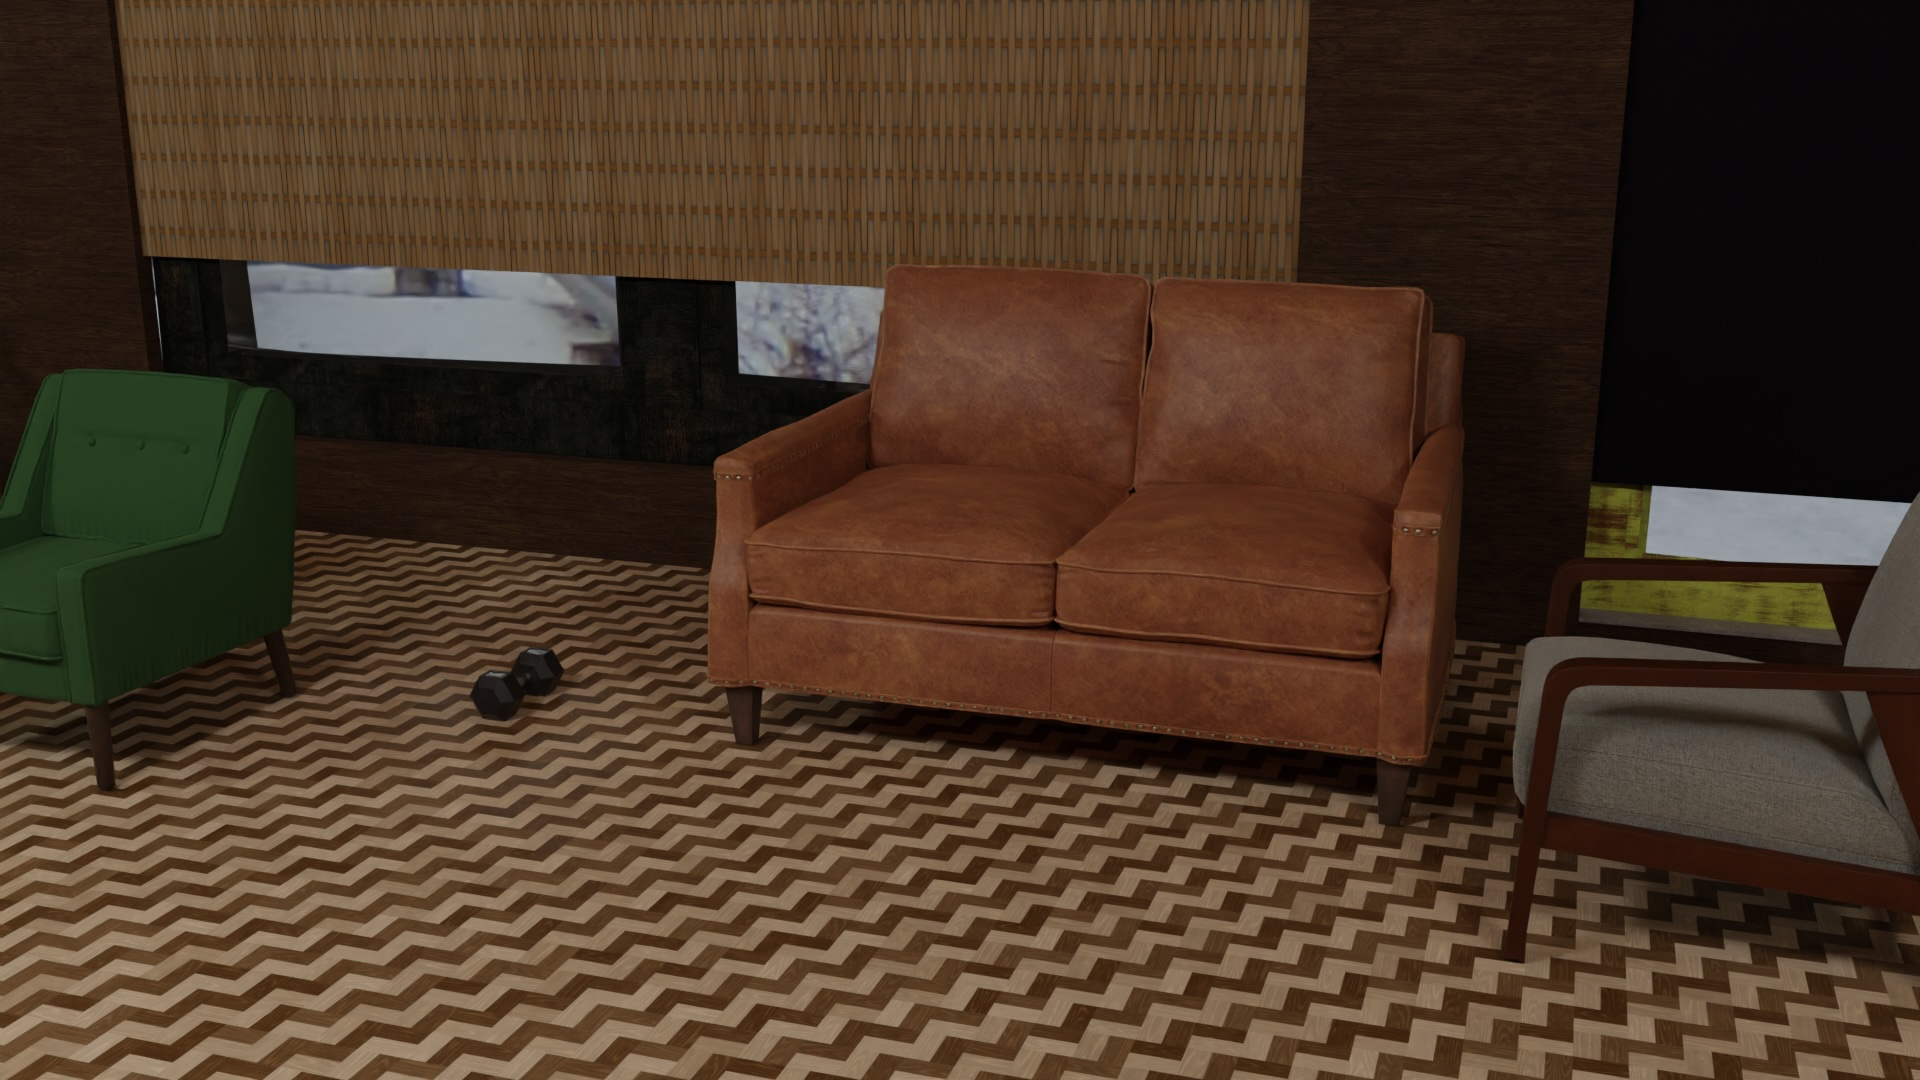
\includegraphics[width=0.24\linewidth]{figs/ase_fly_through_renderings/0041.jpg} 
    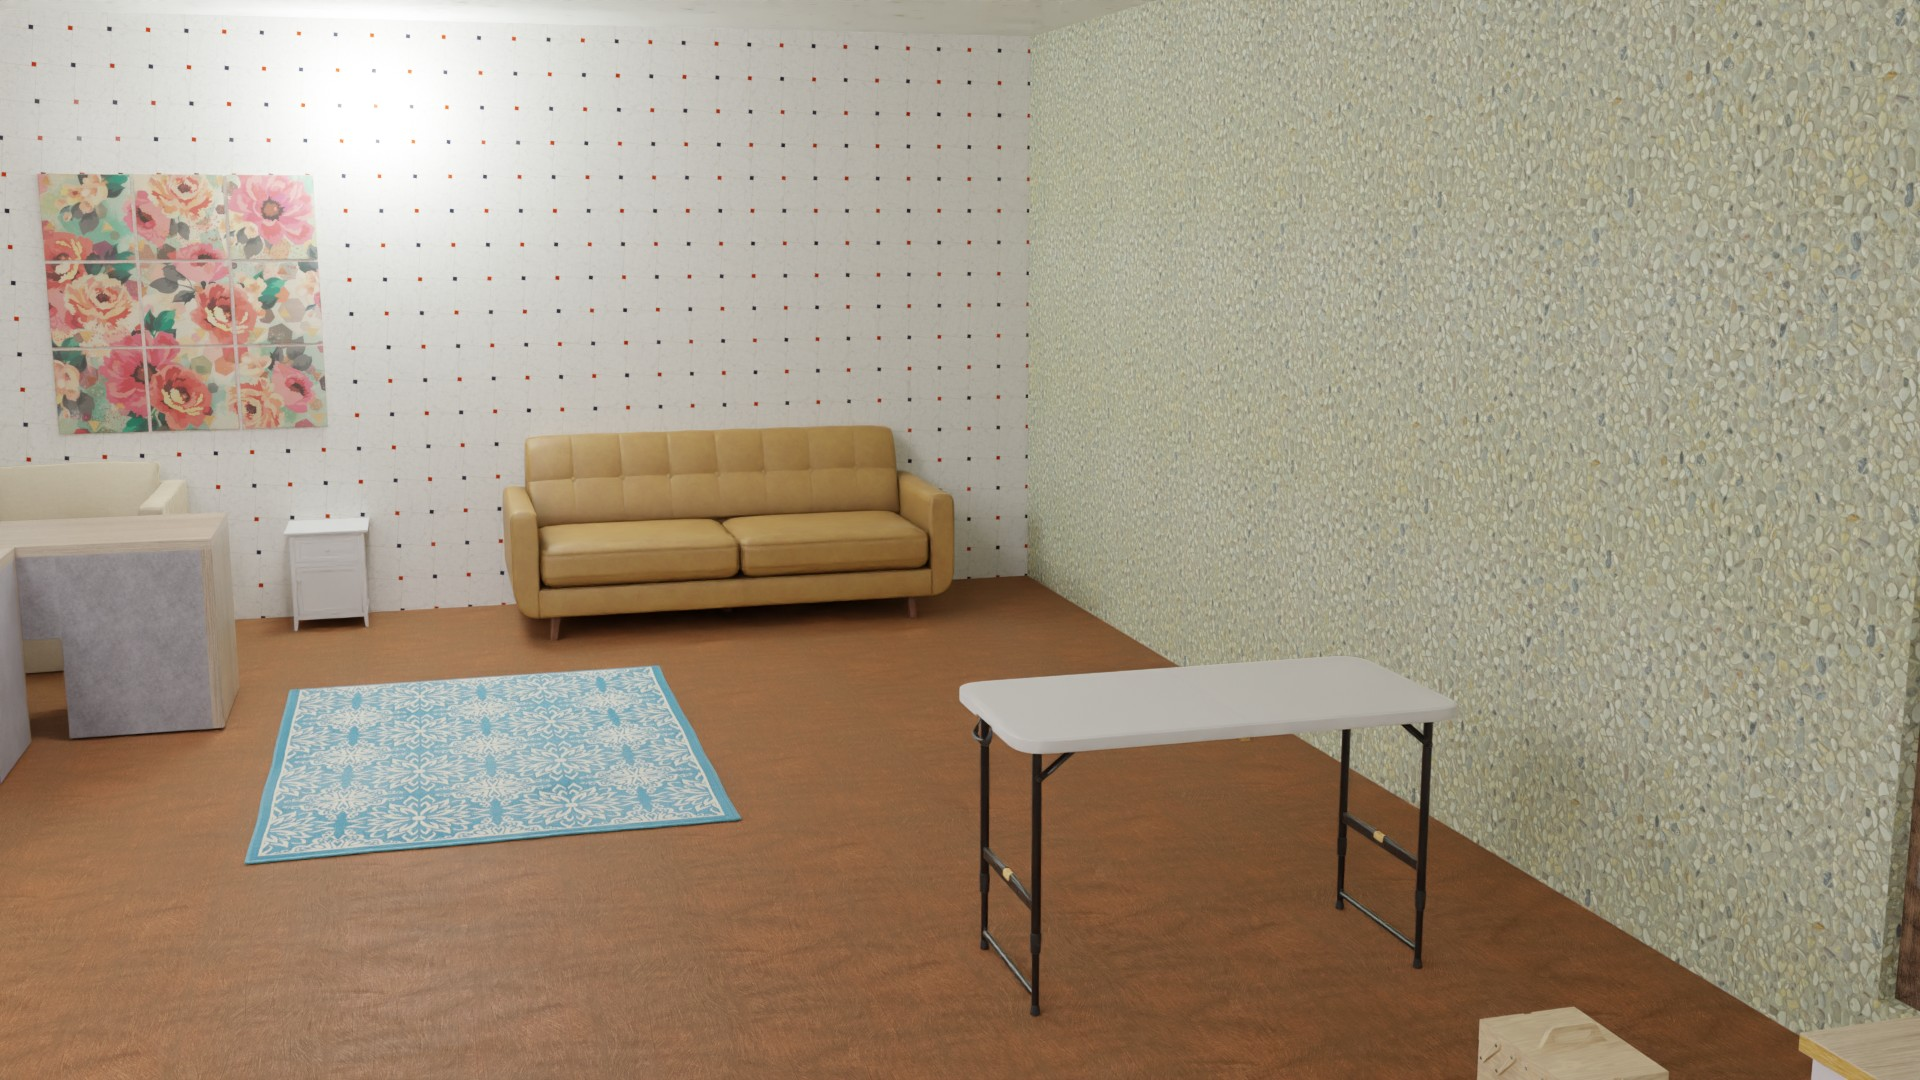
\includegraphics[width=0.24\linewidth]{figs/ase_fly_through_renderings/0099.jpg} 
    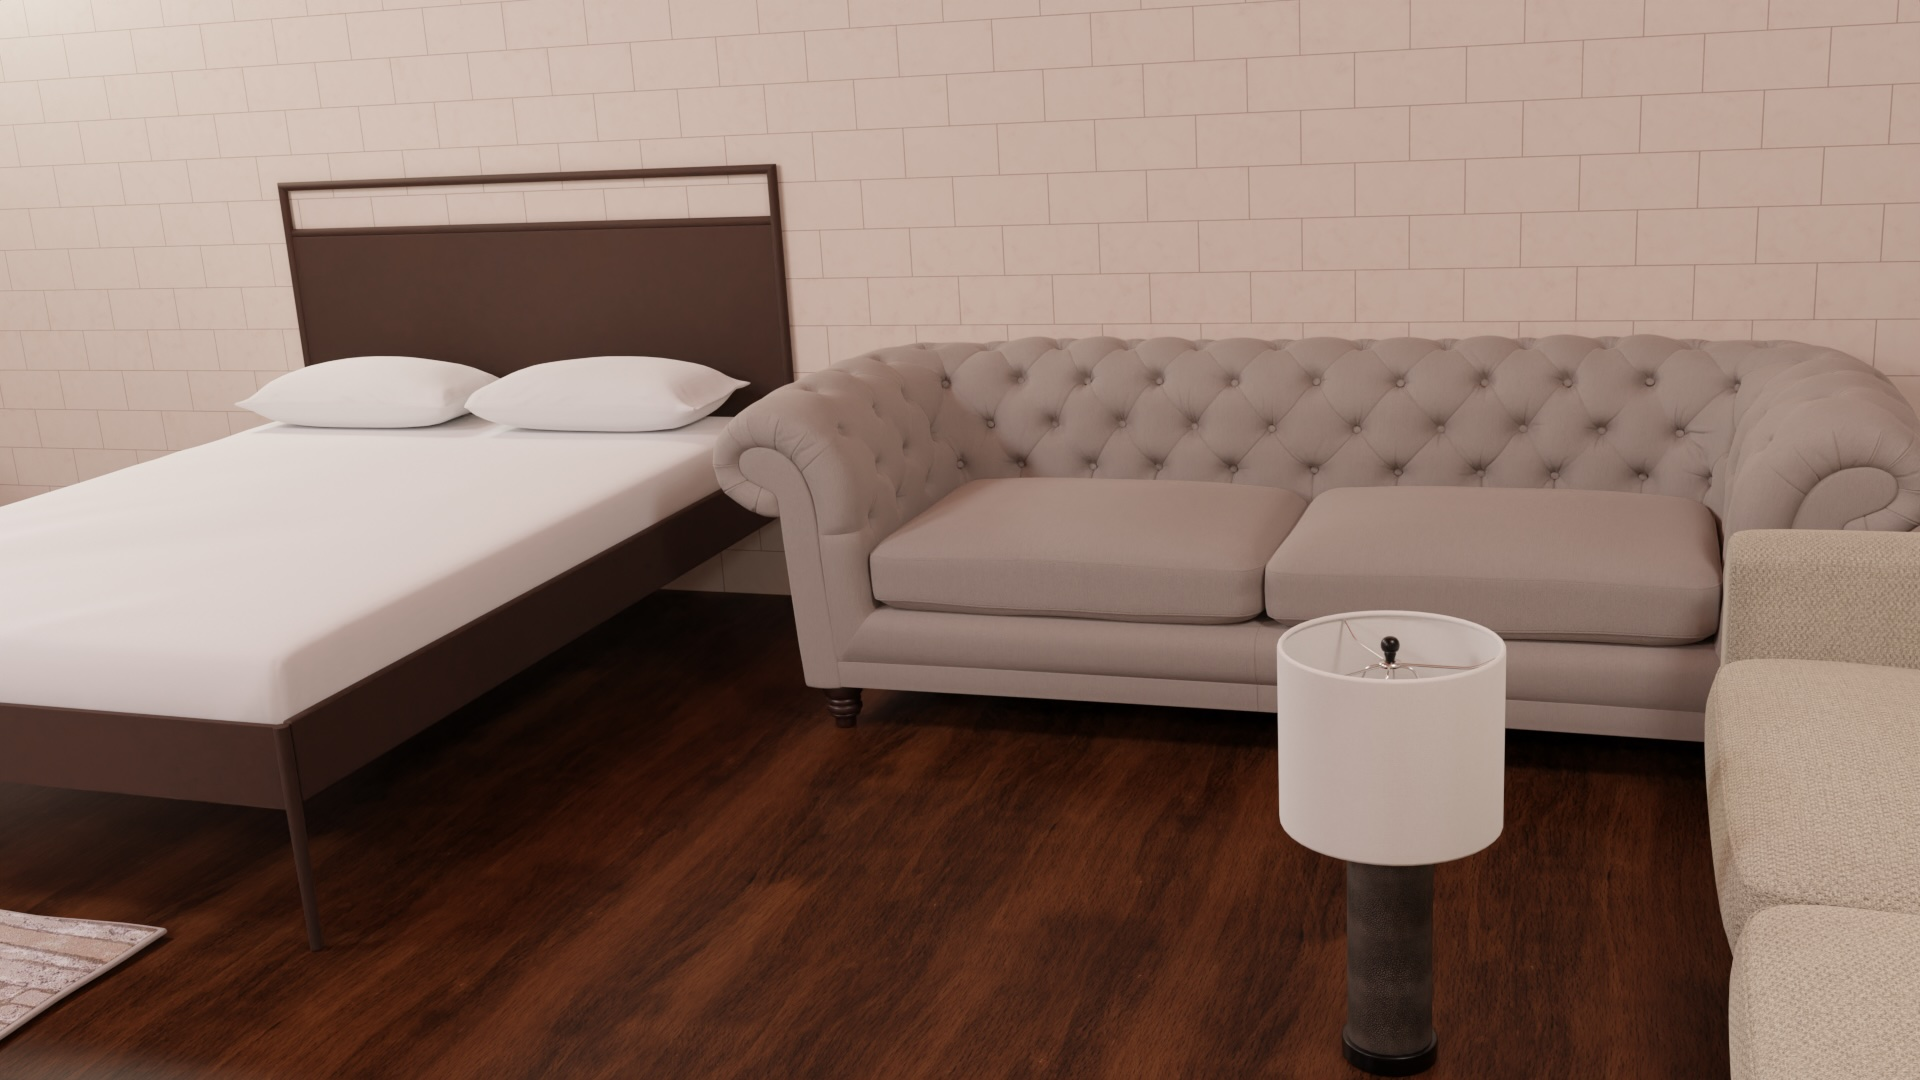
\includegraphics[width=0.24\linewidth]{figs/ase_fly_through_renderings/0152.jpg} 
    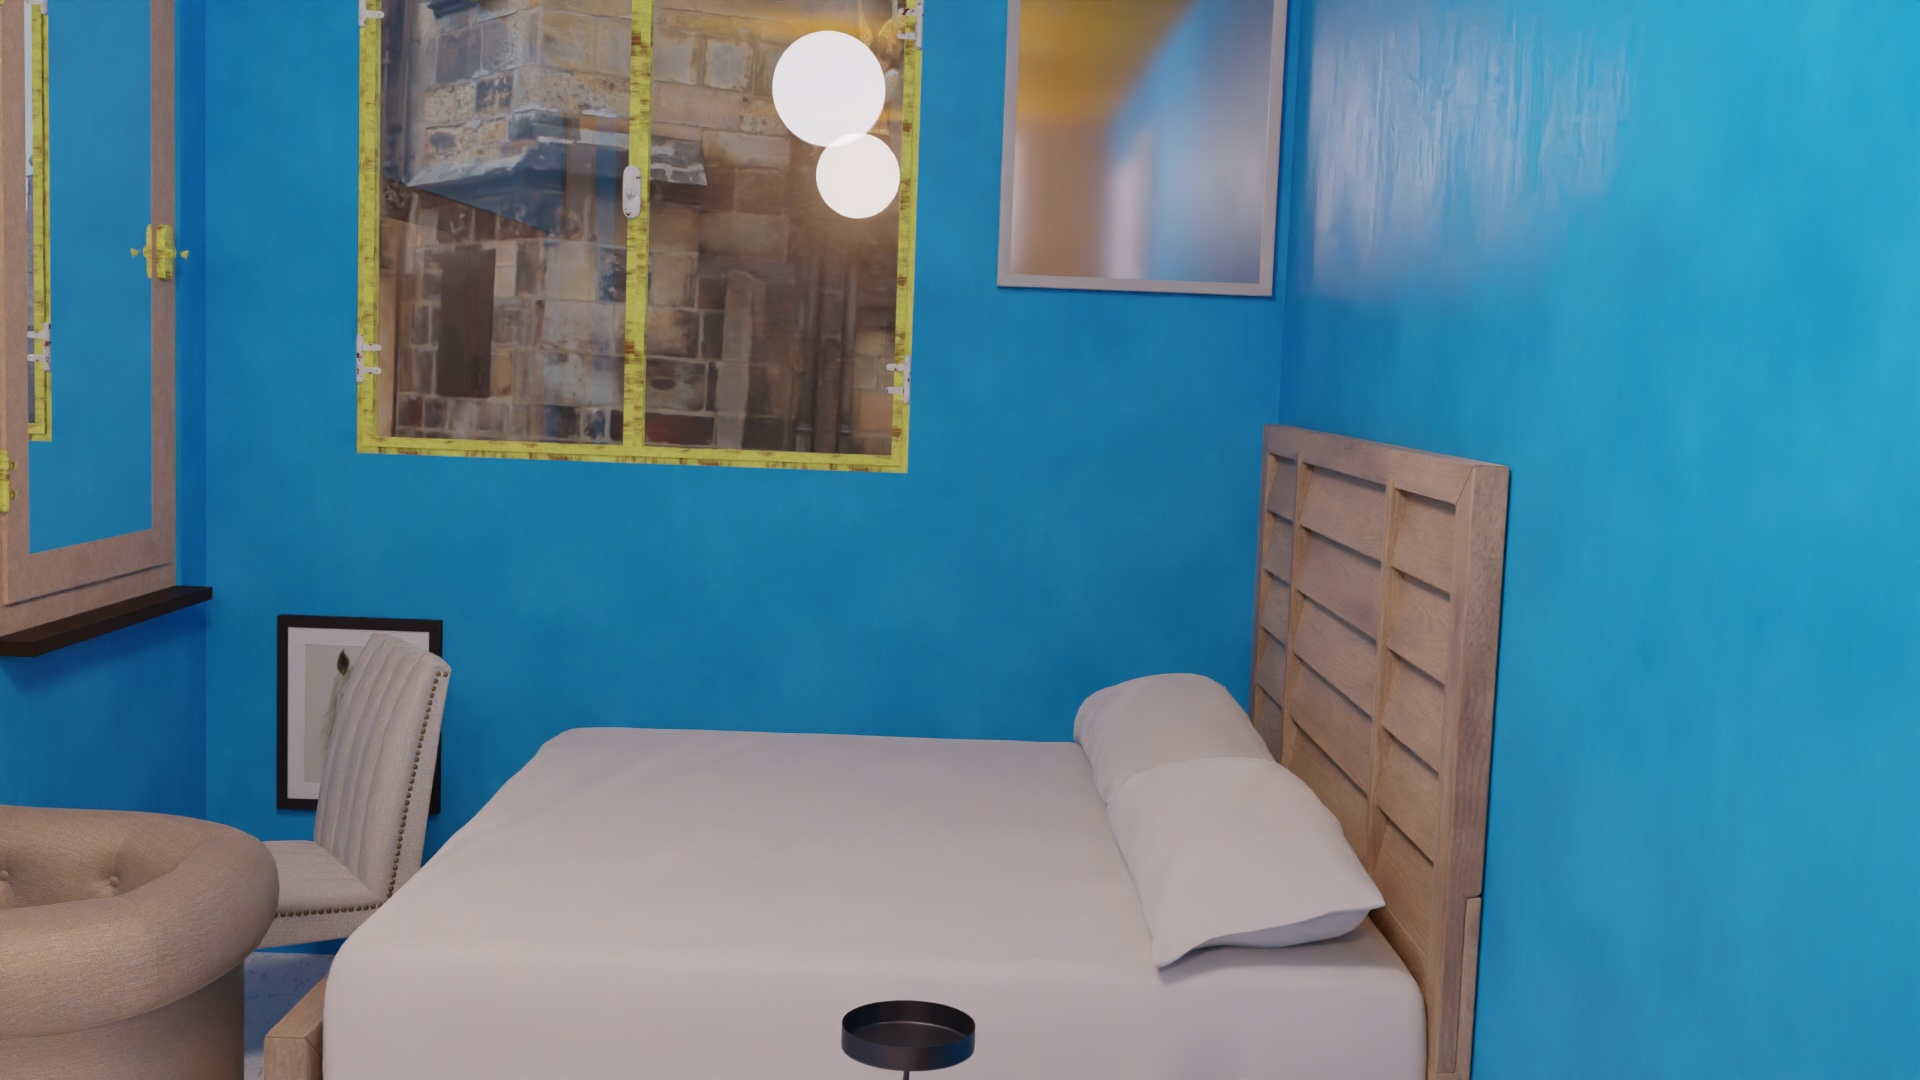
\includegraphics[width=0.24\linewidth]{figs/ase_fly_through_renderings/0754.jpg}
    \caption{Randomly selected scenes from \DatasetName{}.
        (top) Birds eye view renderings 
        demonstrating room layouts and furniture arrangements.
        (bottom) Ego-centric close-up renderings showing scene details.
    }
    \label{fig:dataset_examples}
\end{figure*}
%
%The following subsections provide more details of our synthetic dataset and the visual input data used for model training.

\subsection{Large Scale Training Dataset}

% dataset with examples & annotations
\DatasetName{} consists of $100k$ training pairs
with photo-realistically rendered indoor scenes
coupled with structured language commands.
In addition to these training sequences, \DatasetName{} also provides an additional $1k$ scenes for testing.
Figure~\ref{fig:dataset_examples} presents example scenes from the dataset.
To the best of our knowledge, this is the largest synthetically generated and annotated dataset to date.
%

% which consists of overall $100k$ scenes for training 

Specifically, a training pair for \METHOD~consists of
a 3D scene model represented through a rendered video sequence
(input)
and associated with a sequence of commands (ground truth).
% example training pair
An example training pair for our method is shown in Figure~\ref{fig:training_datum}.
\begin{figure}
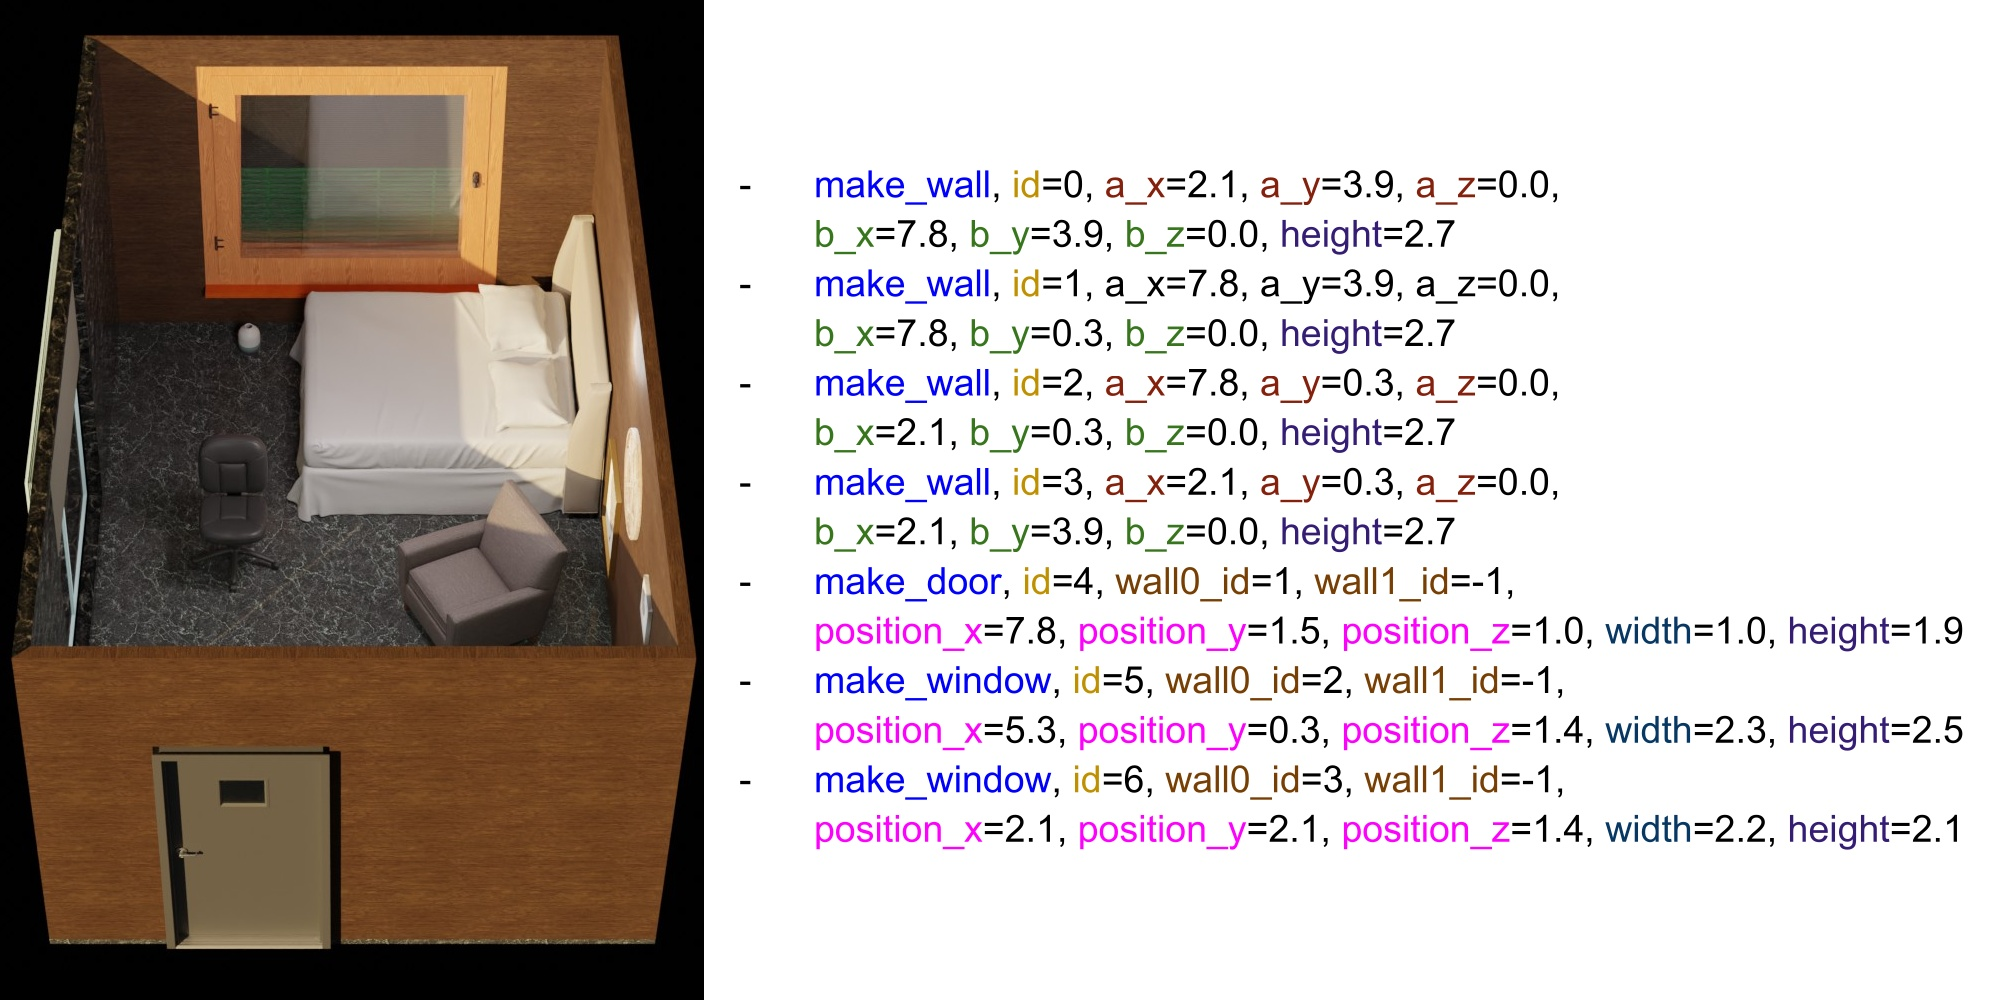
\includegraphics[width=1.0\columnwidth]{figs/sample_training_datum3.jpg}
\caption{Example of training data pair. A scene with objects is shown on the left, while the respective GT \METHOD~language description is shown on the right.}
\label{fig:training_datum}
\end{figure}

\paragraph{Generation.} Each of our synthetic indoor scenes are generated in the following way:
\begin{enumerate}
    \item Start with:
        \begin{itemize}
            \item A floor plan defining the layout of all rooms
            \item A corresponding 3D model (room \& object geometry, materials and illumination)
        \end{itemize}
    \item A trajectory is estimated going through the 3D scene model, simulating an agent walking around wearing an Aria sensor
    \item A photo-realistic RGB rendering of the trajectory is generated with additional annotation data (depth and instance segmentation maps)
    \item A \SLAM-based point cloud inferred from the synthetic video sequence and aligned with the initial 3D scene model/floor plan
\end{enumerate}



% ASE statistics
% Preview source code for paragraph 0

\begin{table}
\small
\begin{centering}
\caption{
    Comparison between existing indoor datasets.
    P-R: Photo-realistic;
    Ego: Ego-centric;
    Camera: Either Fisheye(F) or Pinhole(P), or panorama photo(360);
    Seg: object and layout segmentations rendered to images;
    L-GT: Layout entity ground-truth,
    such as individual wall/window/door parameters.
}
\label{tab:ase_stats}
\resizebox{\linewidth}{!}{%
\begin{tabular}{|c|c|c|ccccccc|c|}
\hline 
Type & Name & Scenes & Trajectory & P-R & Ego & Camera & Depth & Seg & L-GT & License\tabularnewline
\hline 
\hline 
\multirow{7}{*}{Syn} & ASE (\textbf{Ours}) & 100k & \textcolor{green}{$\checkmark$} & \textcolor{green}{$\checkmark$} & \textcolor{green}{$\checkmark$} & F & \textcolor{green}{$\checkmark$} & \textcolor{green}{$\checkmark$} & \textcolor{green}{$\checkmark$} & Agreement needed\tabularnewline
\cline{2-11} \cline{3-11} \cline{4-11} \cline{5-11} \cline{6-11} \cline{7-11} \cline{8-11} \cline{9-11} \cline{10-11} \cline{11-11} 
 & ProcTHOR & 10k & \textcolor{red}{$\times$} & \textcolor{red}{$\times$} & \textcolor{green}{$\checkmark$} & P & \textcolor{green}{$\checkmark$} & \textcolor{green}{$\checkmark$} & \textcolor{green}{$\checkmark$} & Apache2.0\tabularnewline
\cline{2-11} \cline{3-11} \cline{4-11} \cline{5-11} \cline{6-11} \cline{7-11} \cline{8-11} \cline{9-11} \cline{10-11} \cline{11-11} 
 & HyperSim & 461 & \textcolor{green}{$\checkmark$} & \textcolor{green}{$\checkmark$} & \textcolor{green}{$\checkmark$} & P & \textcolor{green}{$\checkmark$} & \textcolor{green}{$\checkmark$} & \textcolor{red}{$\times$} & Special license\tabularnewline
\cline{2-11} \cline{3-11} \cline{4-11} \cline{5-11} \cline{6-11} \cline{7-11} \cline{8-11} \cline{9-11} \cline{10-11} \cline{11-11} 
\cline{2-11} \cline{3-11} \cline{4-11} \cline{5-11} \cline{6-11} \cline{7-11} \cline{8-11} \cline{9-11} \cline{10-11} \cline{11-11} 
 & Structured3D & 3,500 & \textcolor{red}{$\times$} & \textcolor{green}{$\checkmark$} & \textcolor{green}{$\checkmark$} & P & \textcolor{green}{$\checkmark$} & \textcolor{green}{$\checkmark$} & \textcolor{green}{$\checkmark$} & MIT\tabularnewline
\cline{2-11} \cline{3-11} \cline{4-11} \cline{5-11} \cline{6-11} \cline{7-11} \cline{8-11} \cline{9-11} \cline{10-11} \cline{11-11} 
 & SceneNet RGB-D & 57 & \textcolor{green}{$\checkmark$} & \textcolor{green}{$\checkmark$} & \textcolor{green}{$\checkmark$} & P & \textcolor{green}{$\checkmark$} & \textcolor{green}{$\checkmark$} & \textcolor{red}{$\times$} & Special license\tabularnewline
\cline{2-11} \cline{3-11} \cline{4-11} \cline{5-11} \cline{6-11} \cline{7-11} \cline{8-11} \cline{9-11} \cline{10-11} \cline{11-11} 
 & InteriorNet & 10k/1.7M & \textcolor{green}{$\checkmark$} & \textcolor{green}{$\checkmark$} & \textcolor{green}{$\checkmark$} & F, P & \textcolor{green}{$\checkmark$} & \textcolor{green}{$\checkmark$} & \textcolor{red}{$\times$} & Agreement needed\tabularnewline
\hline 
\multirow{3}{*}{Real} & Zillow Indoor & 2,564 & \textcolor{red}{$\times$} & \textcolor{green}{$\checkmark$} & \textcolor{red}{$\times$} & 360 & \textcolor{red}{$\times$} & \textcolor{red}{$\times$} & \textcolor{green}{$\checkmark$} & Apache 2.0\tabularnewline
\cline{2-11} \cline{3-11} \cline{4-11} \cline{5-11} \cline{6-11} \cline{7-11} \cline{8-11} \cline{9-11} \cline{10-11} \cline{11-11} 
 & HM3D & 1,000 & \textcolor{red}{$\times$} & \textcolor{green}{$\checkmark$} & \textcolor{red}{$\times$} & P & \textcolor{green}{$\checkmark$} & \textcolor{red}{$\times$} & \textcolor{red}{$\times$} & MIT\tabularnewline
\cline{2-11} \cline{3-11} \cline{4-11} \cline{5-11} \cline{6-11} \cline{7-11} \cline{8-11} \cline{9-11} \cline{10-11} \cline{11-11} 
 & ScanNet & 1,513 & \textcolor{green}{$\checkmark$} & \textcolor{green}{$\checkmark$} & \textcolor{red}{$\times$} & P & \textcolor{green}{$\checkmark$} & \textcolor{green}{$\checkmark$} & \textcolor{red}{$\times$} & Special license (data)\tabularnewline
\hline 
\end{tabular}
}
\par\end{centering}
\end{table}


%
\paragraph{Dataset Properties.} An overview of properties of existing indoor datasets is given in Table \ref{tab:ase_stats}.
Note that
we define ego-centric as wearing a real camera on the head or chest
or having a synthetic camera with similar trajectory.
In particular, 
we follow the Aria ego-centric specifications \cite{aria_white_paper}.
Also note that
\emph{InteriorNet} contains 15k sequences 
rendered from 10k randomly selected layouts and
5M images from 1.7M randomly selected layouts,
with 3 images per layout.
%
\DatasetName{} is especially useful for machine learning tasks not just due to its sheer scale (allowing algorithms to generalize well), but also the wide variety of available ground truth annotations.
For example, the layout ground truth (L-GT) is critical for training \METHOD,
but not included in the majority of other datasets.

\DatasetName{} is made publicly available to the research community.
Users must agree to a standard licence to prevent data misuse
and it is to be used for non-commercial purposes only.


\subsection{Semi-dense Point Clouds from Video Sequences}

We utilize the open-source Machine Perception Services (MPS) from Project Aria~\cite{AriaMPS2023} to estimate a SLAM trajectory and generate a point cloud map of the scene. Similarly to LSD-SLAM \cite{engel14eccv} they maximize the extracted geometric information from a video sequence by estimating points for all image regions with non-negligible gradient. Each point is parameterized by an inverse distance and its associated Gaussian uncertainty in the frame in which it is first observed. KLT-based \cite{tomasi1991detection} epipolar line-searches in subsequent frames provide sub-pixel accurate short and large-baseline measurements that are absorbed using a Kalman filter update. While points are associated with a final estimated uncertainty, they consider utilizing this information in a probabilistically-sound way as beyond the scope of their work, and instead choose to sub-select points whose uncertainty is below a predefined threshold.

%\subsection{Input Data from Other Sources}
% 
%It is important to highlight that the generation of the input point clouds is not restricted to outputs from Project Aria Machine Perception Services. Alternatively, one can utilize off-the-shelf mobile phones and other commodity frameworks, such as the COLMAP structure-from-motion package\cite{schoenberger2016sfm}, to produce the necessary inputs.

\section{Structured Language Commands}
\label{sec:parameters_supp}

Command parameters can have data types such as \lstinline[style=dtypestyle]!float! or \lstinline[style=dtypestyle]!int!. The full list of parameters for each command can be found in Table~1 of the main paper. Below, we provide detailed descriptions of each parameter:


\begin{itemize}
\item Wall parameters
    \begin{itemize}
    \small
        \item \lstinline[style=cmdstyle]!id!: The ID of the wall.
        \item \lstinline[style=cmdstyle]!(a_x,a_y,a_z) / (b_x,b_y,b_z)!: The $x,y,z$ coordinates of the first / second corner of the wall.
        \item \lstinline[style=cmdstyle]!height!: The height of the wall. Note that we assume the walls are straight and gravity-aligned.
    \end{itemize}
    
\item Door/Window parameters
    \begin{itemize}
    \small
        \item \lstinline[style=cmdstyle]!id!: The ID of the door/window.
        \item \lstinline[style=cmdstyle]!wall0_id,wall1_id!: The IDs of the (potentially two) walls that a door/window is attached to.
        \item \lstinline[style=cmdstyle]!position_x,position_y,position_z!: The $x,y,z$ coordinates of the centre of the door/window.
        \item \lstinline[style=cmdstyle]!width, height!: The width and height of the door/window.
    \end{itemize}
\end{itemize}
    

\section{Network Architectures}
\label{sec:architecture}
%
\subsection{Point Cloud Encoder}
\label{subsec:point_cloud_encoder}

The point cloud encoder is essentially a ResNet-style~\cite{he2016deep} encoder that employs sparse 3D convolutions~\cite{tang2020searching,tang2022torchsparse} in place of standard 3D convolutions. It uses a total of 5 down convolutional layers with a kernel size of 3 and a stride of 2. This architecture effectively reduces the number of points (i.e. active sites) by $\approx 1000$. As a result, the feature sizes are manageable in terms of size and can be used effectively in the subsequent Transformer decoder~\cite{vaswani2017attention}. The point cloud encoder consists of $\approx 20M$ optimizable parameters, which contribute to its capacity and ability to capture intricate geometric information.

\subsection{Transformer Decoder}
\label{app:decoder}

Our implementation includes a transformer decoder consisting of 8 layers, each with 8 heads for multi-head attention, and a feature dimension of $512$. This configuration results in a relatively modest set of $\approx 35M$ parameters. Our vocabulary size is $2048$, which we also use as the maximum sequence length of tokens. While we could theoretically increase the vocabulary size to accommodate a larger number of tokens, in practice the majority of the released rendered scenes can be accurately represented using significantly fewer tokens than $2048$. 

In some scenarios, we employ nucleus sampling~\cite{holtzman2019curious} with a top-p probability mass during autoregressive inference. By using nucleus sampling, we limit the selection of next tokens to a subset with a cumulative probability threshold, allowing for greater exploration at inference time. Quantitative results are decoded greedily.

\section{Training Methodology}

We use the AdamW optimizer 
with a default initial learning rate of $10^{-4}$ and
weight decay as well as dropout enabled.
For the image-only Raytran-based encoder model~\cite{tyszkiewicz2022raytran},
we found that an initial learning rate of $10^{-3}$ provided better convergence.
We train all our methods with an effective batch size of 64, which may be distributed across multiple nodes. 
During training, the only augmentations we perform are: 1) up to 360 degrees of rotation around the z-axis (since the scenes are assumed to be gravity-aligned), and 2) random subsampling of point clouds up to a specificed maximum number of points (500k). 
Training times lasted approximately between 3 and 4 days. 

Our training loss is the standard cross-entropy loss on next token prediction, similar to how most LLMs are trained ~\cite{openai2023gpt4,sutskever2014sequence}. 



%
\section{Tokenization Details}

The conversion of a parameter $\textbf{\texttt{x}}$ into an integer token $\textbf{\texttt{t}}$ is determined by two factors: its data type and its magnitude. In general, parameters with \lstinline[style=dtypestyle]!int! and \lstinline[style=dtypestyle]!bool! data types are converted using the $\textbf{\texttt{t = int(x)}}$ operation. For \lstinline[style=dtypestyle]!float! parameters, the conversion involves $\textbf{\texttt{t = round(x/res)}}$, where $\textbf{\texttt{res}}$ represents the resolution. 
Note that  by designing the \METHOD~language,
we also design the tokenization.
This is notably different from standard NLP tokenization,
which involves \emph{B}yte-\emph{P}air \emph{E}ncodings (\emph{BPE}) \cite{openai2023gpt4}.




\section{Additional Results: Layout Prediction}
In this section,
we present additional qualitative results,
comparisons with related works and
more evaluations with respect to extending \METHOD{}.

\begin{figure}[t]
    \centering
    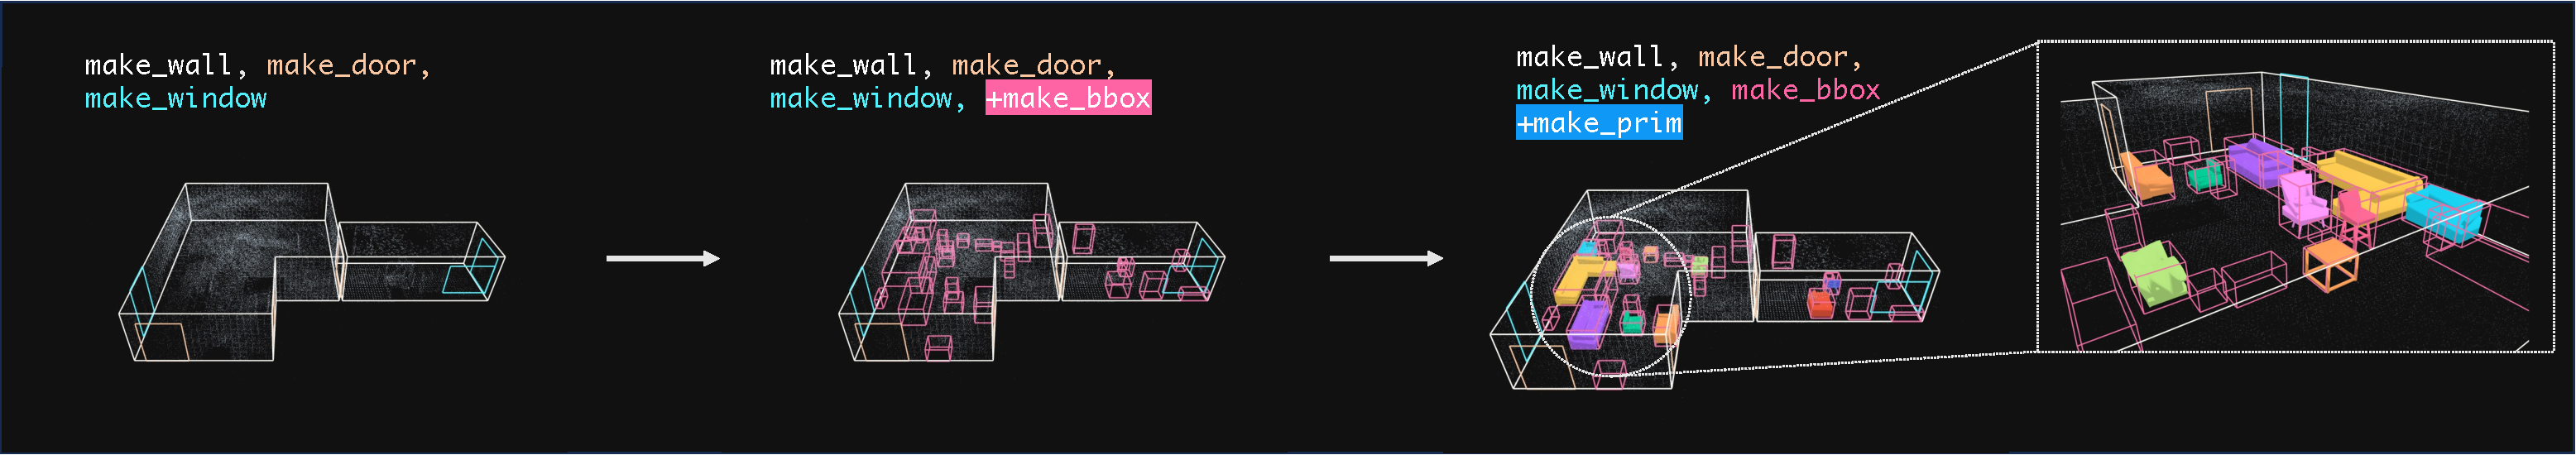
\includegraphics[width=\columnwidth]{figs/commands_wide.pdf}
    \caption{
        An illustrative example of how the expressiveness of SceneScript's reconstruction increases through the addition of new commands.
        (left) Layout commands only: walls, doors and windows.
        (middle, left) Addition of \texttt{make\_bbox} enriches the scene reconstruction with bounding boxes for detected objects.
        (middle, right) Addition of \texttt{make\_prim} adds volumetric primitives for detected chairs, sofas and tables.
        (right) Close-up illustrating the fidelity possible with just these five commands.
    }
    \label{fig:commandVisExamples0}
\end{figure}

\subsection{Visualization of High-Level Commands}

% example to highlight the various commands separately
Figure \ref{fig:commandVisExamples0} presents a visual example of how the fidelity of \METHOD's reconstruction can be increased through the addition of new commands. 
% the structured language commands we use to describe indoor scenes. 
Initially, structural room layouts are represented by three commands: \texttt{make\_wall}; \texttt{make\_door}; and \texttt{make\_window}.
Just through the addition of \texttt{make\_bbox}, scene content is now present in the reconstruction in the form of object detections.
Finally for the commands discussed in the main paper, \texttt{make\_prim} for the three selected target classes enables not just the capture of the scene's overall structure and content, but also much finer reconstruction of scene objects themselves. 

Importantly, each of these levels of detail is enabled without change to \METHOD's network architecture, and instead just by increasing the expressiveness of the structured language it infers.

Note that
the volumetric primitive commands for detected objects are a proof of concept.
We trained our models for the object primitive commands only on a subset
of the available object types from the \DatasetName{}.
Supported object class labels are ``\emph{chair}'', ``\emph{sofa}'' and ``\emph{table}''.
Objects with these labels are modeled by cuboid and cylinder primitives.
Detected bounding boxes of object instances with unsupported classes remain empty.
%


\begin{figure}[t]
    \centering
    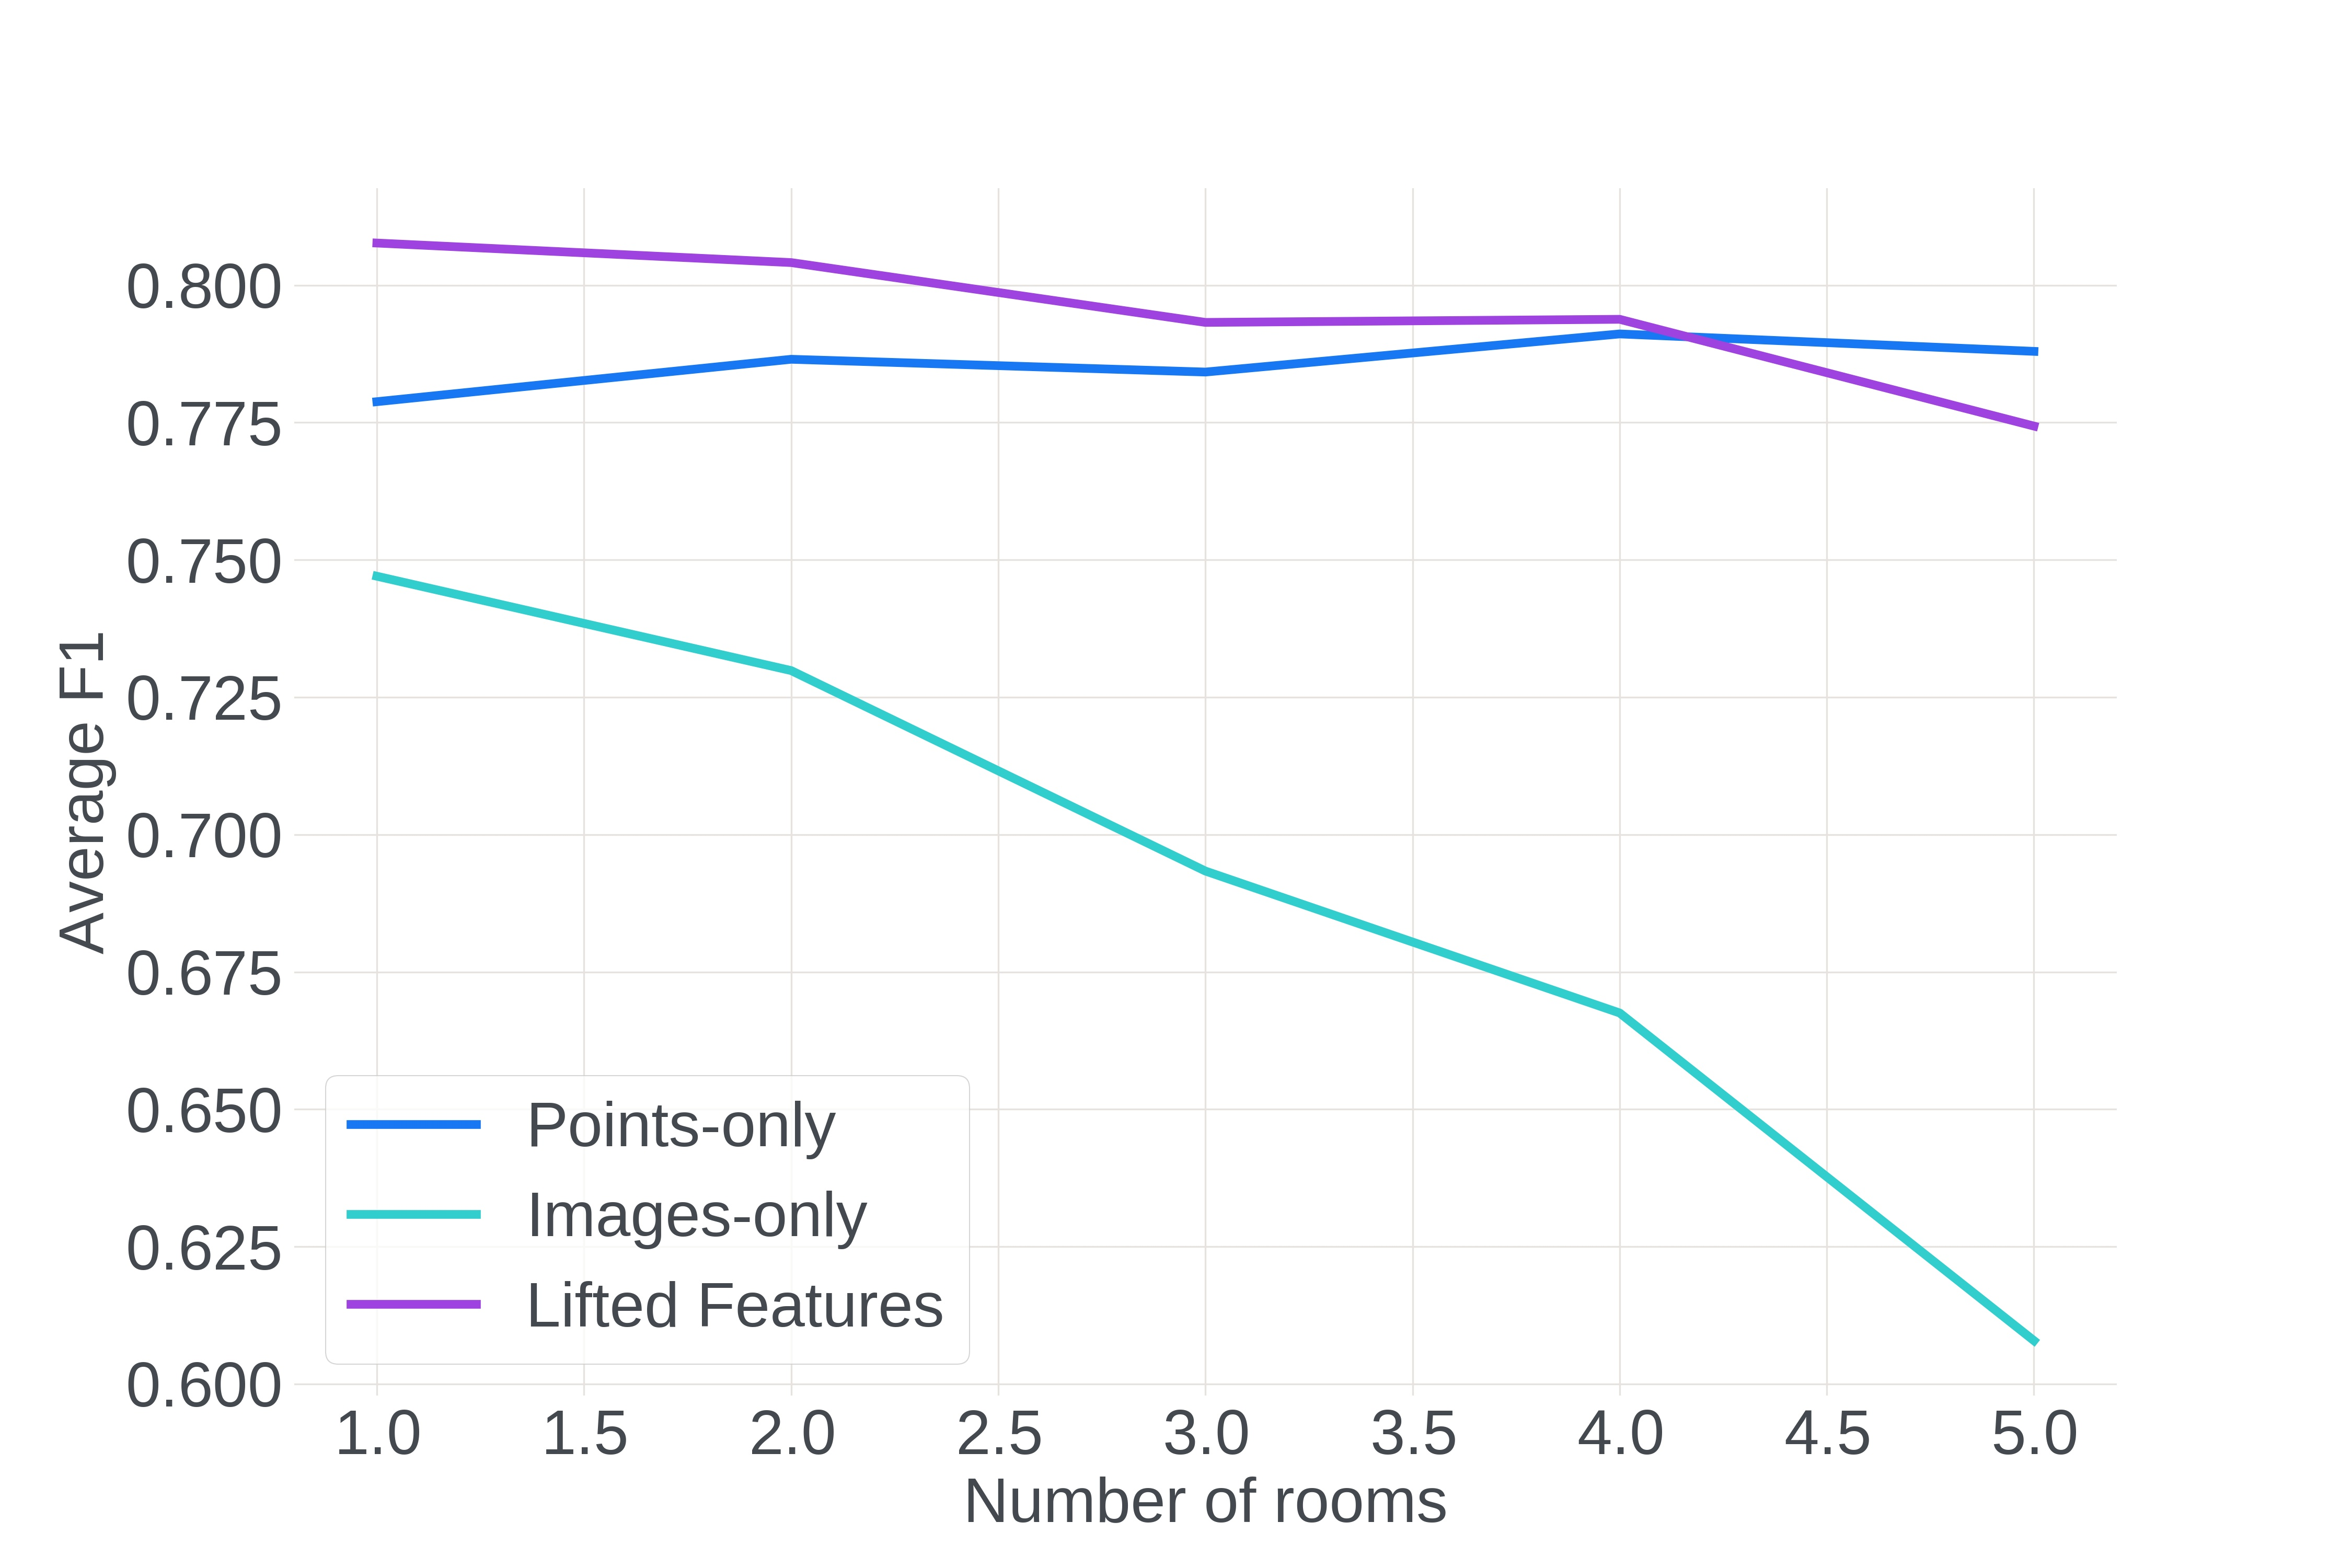
\includegraphics[width=0.5\columnwidth]{figs/roomsvsf1.jpg}
    \caption{
        F1-Score model performance graphs
        for our various encoder variants
        as functions of the number of rooms in a scene.
    }
    \label{fig:roomsf1}
\end{figure}
\label{subsec:failure_cases}
\begin{figure}[h]
    \centering
    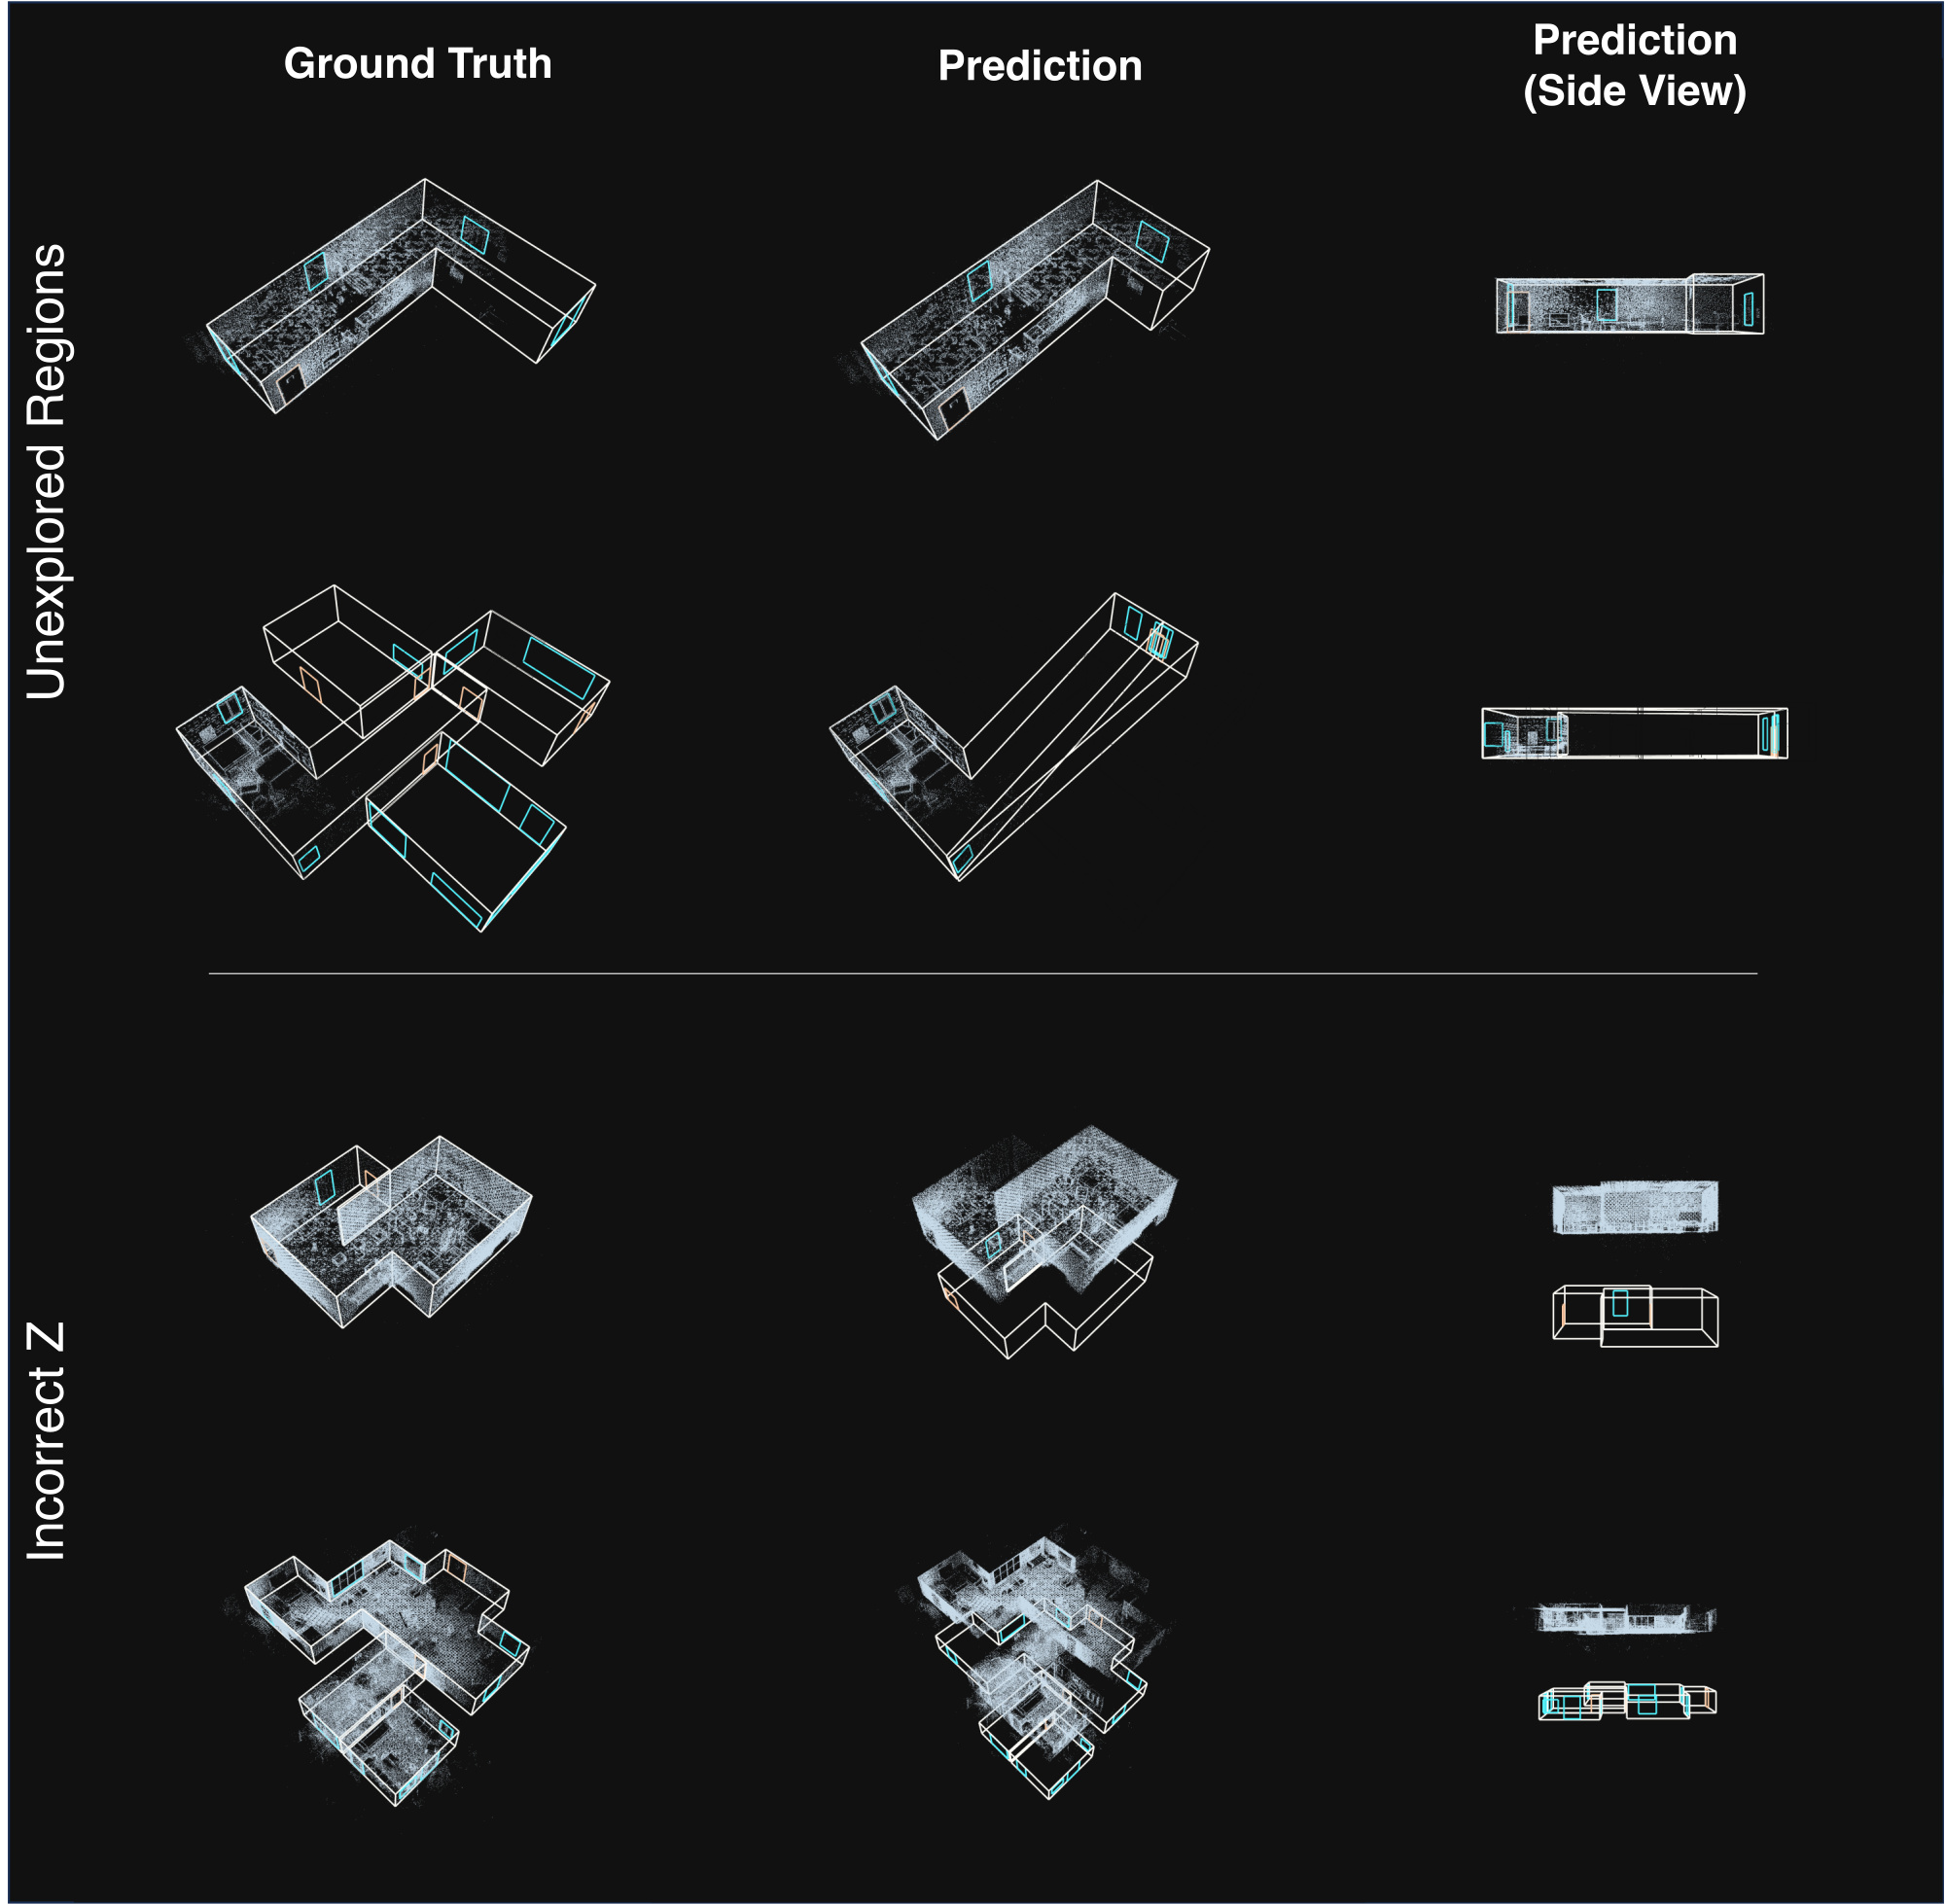
\includegraphics[width=0.8\columnwidth]{figs/failures.jpg}
    \caption{Examples from two notable failure types observed in \METHOD predictions. (top) Limited exploration of the scene makes the ground truth difficult, or in some cases potentially impossible to predict. (bottom) Accurate overall room structure is predicted, but at an incorrect Z value.}
    \label{fig:failures}
\end{figure}

\subsection{Model Performance with respect to Scene Complexity}
\label{app:num_rooms}

The Average F1-score graphs of Figure \ref{fig:roomsf1} demonstrate
the performance of our \METHOD{} model with varying encoders
as a function of the number of rooms in a scene.
Our \METHOD{} model performs constantly well 
when inputting points only or lifted features.
As opposed to this, 
performance drops drastically with increasing room number
when encoding scenes only using images.
We posit that the decrease in performance is due to
the model's lack of occlusion reasoning.
With increasing number of layout elements,
the rays linked to image observations traverse
more scene space by going
through a higher number of rooms
when ignoring wall intersections.
This likely results in 
our model falsely attending to occluded image observations.


\subsection{Failure Cases}

%
In this section, we detail observed failure types for the task of layout estimation on \DatasetName{}.
Aside from expected errors such as slightly incorrect wall corner, window and door placement, or entirely missed, we observe two notable failure modes for \METHOD.

The more common of the two occurs due to non-complete exploration of the target scene. In this scenario there are significant portions of the scene structure that are poorly observed, potentially not at all, making the ground truth structure near unpredictable.

An especially interesting failure mode is the reconstruction of accurate room structure, but at an incorrect Z-value. For the point cloud-based encoder configurations, we suspect that this failure mode is caused by particular sensitivity to noise to point outliers in the Z-direction. This failure mode is also observed in the image-only encoder configuration, suggesting it also exhibits more sensitivity to in the Z direction than XY.

We visualize a couple of examples for each of these failure types in Figure~\ref{fig:failures}. Worth noting is that this figure is comprized of scenes taken from the worst 10 predictions out of the 1000 scene test set, as defined by wall entity distance. Therefore, while clearly illustrating the failures described, they should not be taken as representative of general prediction quality.



\begin{table}
\centering
% \resizebox{\linewidth}{!}{%
    \caption{
    Accuracy reported as raw entity distance for the encoder setups tested for \METHOD. 
    }
\begin{tabular}{c|cc|cc|cc}
        & \multicolumn{6}{c}{Entity Distance (cm)} \\
        \hline
         & \multicolumn{2}{c|}{Wall} & \multicolumn{2}{c|}{Door} & \multicolumn{2}{c}{Window}\\
        Method & med. & p90 & med. & p90 & med. & p90 \\
        \hline \hline
        Point Cloud &       4.7 & 7.2   & 5.0 & 6.7     & 6.9 & 37.6 \\
        Lifted Features &   4.8 & 7.1   & 4.8 & 6.1     & 5.9 & 26.2  \\
        Image-only &        6.7 & 17.3  & 5.8 & 8.9     & 9.0 & 45.7 \\
    \end{tabular}
    % }
    \label{table:plane_distances}
\end{table}
\subsection{Quantitative Evaluation of Layout Predictions}
\label{app:per_entity}

We include an additional breakdown of the entity distance accuracy metrics in Table~\ref{table:plane_distances}. 
This breakdown of accuracy makes apparent that the improvement offered by lifting image features onto the semi-dense point cloud comes largely in the prediction of windows and doors.
Following the same trend as the results included in the main paper, we observe that windows appear to be the most challenging class to predict accurately. 
However in spite of this challenge, the 90th percentile of window predictions falls within 0.5m of the ground truth for all encoder setups tested.





\section{Additional Results: Object Detection}

\subsection{Implementation Details}
\subsubsection{Training Details of \METHOD{}.}
%
As outlined in the paper, a significant advantage of \METHOD{} lies in its seamless adaptability to other tasks through the addition of new language commands. Here, for instance, we integrate \texttt{make\_bbox} to denote 3D oriented bounding boxes.

Notably, no architectural changes to \METHOD{} have been implemented to facilitate training for object detection. We utilize the point cloud encoder and language decoder detailed in Section \ref{sec:architecture}. The entire training objective is a single cross-entropy loss, which stands as the de facto-standard in training LLMs. The model is trained for $\approx 200k$ iterations using an effective batch size of 64. For this experiment, we only trained a point cloud version of SceneScript.



\subsubsection{Baseline Implementation Details.}

We list implementation details for each method below:
 

\paragraph{3DETR~\cite{misra2021end}:} We downloaded the weights for both 3DETR and 3DETR-m, trained for 1080 epochs on ScanNet, from the official Github repository. We evaluated both models on each ScanNet validation examples, subsampled to $40k$ points. Predictions were thresholded at probability 0.5. We attemped to run NMS in 3D, but achieved worse results, thus the numbers reported in the main paper do not include NMS.

We trained 3DETR (not 3DETR-m) on \DatasetName{} using almost the same configuration as trained on ScanNet. The differences include: a batch size of 128, a PointNet set aggregation downsampling to 4096 (compared to 2048 for ScanNet), 512 furthest point samples as detection queries (compared to 256 for ScanNet), and 200k points per example. 
    
\paragraph{Cube R-CNN~\cite{brazil2023omni3d}:} This method predicts 3D bounding boxes from a single RGB image. To obtain 3D bounding box predictions for an entire scene, we accumulate per-frame predictions via a matching-based tracker. At a high-level, we match predictions of the same class between frames with Hungarian matching with a cost based on IoU and bounding box distances. Then the final bounding box parameters are computed as a running average of the matched and tracked predictions. For evaluation, the accumulated predicted boxes were thresholded at probability 0.5.

\paragraph{ImVoxelNet~\cite{rukhovich2022imvoxelnet}:} This model predicts 3D bounding boxes from a set of RGB images. We trained this method using 10 consecutive frame snippets from \DatasetName{}. During evaluation, we run the model on overlapping 10-frame snippets and apply the same bounding box tracker as described for Cube R-CNN. For evaluation, the accumulated predicted boxes were thresholded at probability 0.1.
    
\paragraph{SoftGroup~\cite{vu2022softgroup}:} Since this is primarily a 3D semantic instance segmentation method, we extract axis-aligned bounding boxes from the predictions by utilizing the predicted instance masks and computing the \textit{minimum} and \textit{maximum} extents of the point set belonging to each instance. The geometric mean of these extents serves as the box center, and the difference between the maximum and minimum extents provides the box scale. Since the bounding boxes are intended to be axis-aligned, the angle is kept at 0. By combining this information with the predicted semantic class, one can conduct evaluations over 3D bounding boxes. We used a publically available checkpoint provided by the authors to conduct inference and extract bounding boxes for evaluation following the aforementioned procedure. 

Note that for ScanNet~\cite{dai2017scannet}, we use the axis-aligned bounding boxes for ground truth as extracted in~\cite{misra2021end,qi2019deep}.

\subsection{Sparse Encoder with 3DETR Head}
\label{subsec:sparsecnn_threedetr}

\begin{table}[h]
\centering
    \caption{Replacing the 3DETR encoder with a SparseCNN results in better performance on \DatasetName.}
    \begin{tabular}{c|c|cc}
        & & \multicolumn{2}{c}{F1} \\
         Method & Input & @.25 IoU & @.50 IoU \\
        \hline \hline
        3DETR '21~\cite{misra2021end} & Points & 0.201 & 0.078 \\
        SparseCNN~\cite{tang2022torchsparse} + 3DETR~\cite{misra2021end} & Points & 0.381 & 0.191 \\
    \end{tabular}
    \label{tab:sparsecnn_3detr}
\end{table}

We run an experiment that confirms that 3DETR's standard settings are well-suited to ScanNet~\cite{dai2017scannet} and SUN RGB-D~\cite{song2015sun}, but perform poorly on \DatasetName{}. For this experiment, we use the same sparse point cloud encoder that SceneScript uses (see Section~\ref{subsec:point_cloud_encoder}) while using the 3DETR decoder. Similar to the pure 3DETR model trained on \DatasetName{}, we increased the number of detection queries to 512, and used 200k points per example for training. We denote this model as SparseCNN+3DETR. Due to lack of resources, this model was only partially trained.

In Table~\ref{tab:sparsecnn_3detr}, we show that replacing 3DETR's Transformer encoder with a sparse CNN encoder~\cite{tang2022torchsparse,tang2020searching} results in stronger performance. We hypothesis that this is due to the non-uniformity of the point clouds arising from Project Aria's semi-dense point clouds from its Machine Perception Services~\cite{AriaMPS2023}. The first two columns of Figures~\ref{fig:ase_bbox_qualitative} and~\ref{fig:ase_bbox_qualitative_iou} qualitatively demonstrates more accurate predictions with this encoder replacement.


\begin{figure}[t]
    \centering
    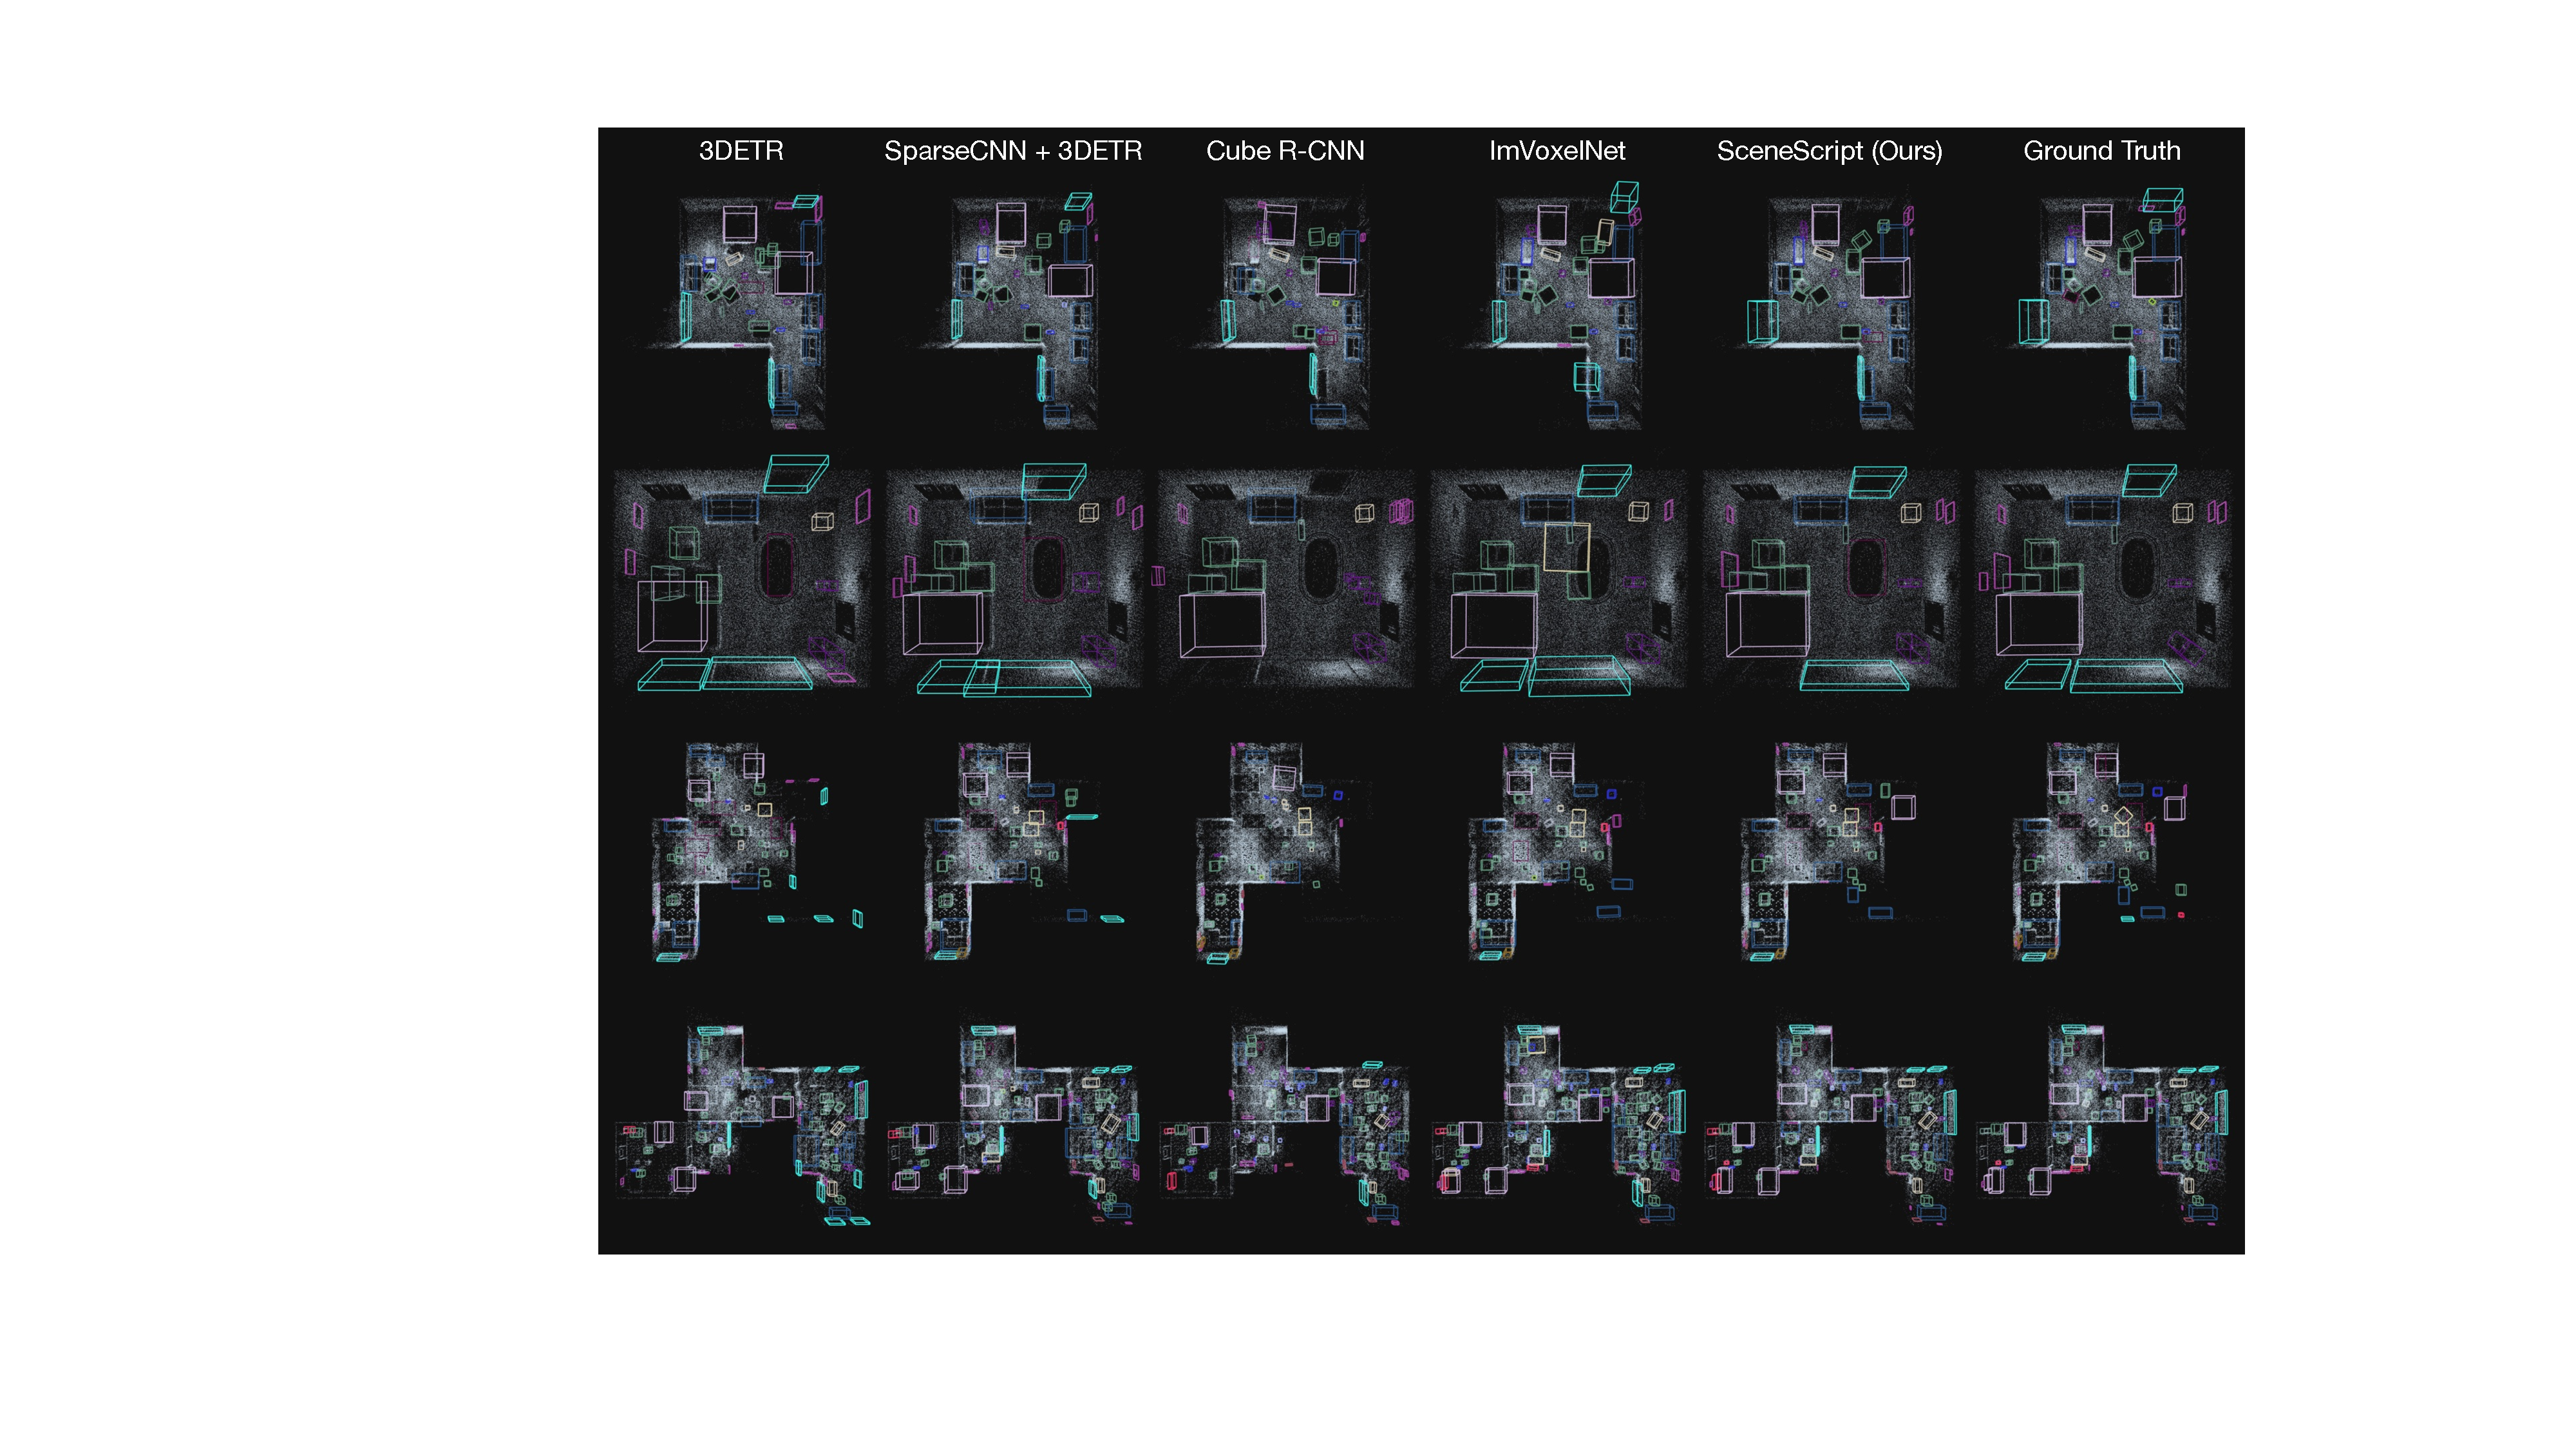
\includegraphics[width=\columnwidth]{figs/ase_bbox_qualitative_compressed.pdf}
    \caption{Qualitative results of predicted bounding boxes on \DatasetName{}. Each bounding box is colored by its class. The colors are: \textcolor{table_bbox_color}{table}, \textcolor{sofa_bbox_color}{sofa}, \textcolor{shelf_bbox_color}{shelf}, \textcolor{chair_bbox_color}{chair}, \textcolor{bed_bbox_color}{bed}, \textcolor{floor_mat_bbox_color}{floor\_mat}, \textcolor{exercise_weight_bbox_color}{exercise\_weight}, \textcolor{cutlery_bbox_color}{cutlery}, \textcolor{container_bbox_color}{container}, \textcolor{clock_bbox_color}{clock}, \textcolor{cart_bbox_color}{cart}, \textcolor{vase_bbox_color}{vase}, \textcolor{tent_bbox_color}{tent}, \textcolor{flower_pot_bbox_color}{flower\_pot}, \textcolor{pillow_bbox_color}{pillow}, \textcolor{mount_bbox_color}{mount}, \textcolor{lamp_bbox_color}{lamp}, \textcolor{ladder_bbox_color}{ladder}, \textcolor{fan_bbox_color}{fan}, \textcolor{cabinet_bbox_color}{cabinet}, \textcolor{jar_bbox_color}{jar}, \textcolor{picture_frame_bbox_color}{picture\_frame}, \textcolor{mirror_bbox_color}{mirror}, \textcolor{electronic_device_bbox_color}{electronic\_device}, \textcolor{dresser_bbox_color}{dresser}, \textcolor{clothes_rack_bbox_color}{clothes\_rack}, \textcolor{battery_charger_bbox_color}{battery\_charger}, \textcolor{air_conditioner_bbox_color}{air\_conditioner}, \textcolor{window_bbox_color}{window}.}
    \label{fig:ase_bbox_qualitative}
\end{figure}

\begin{figure}[t]
    \centering
    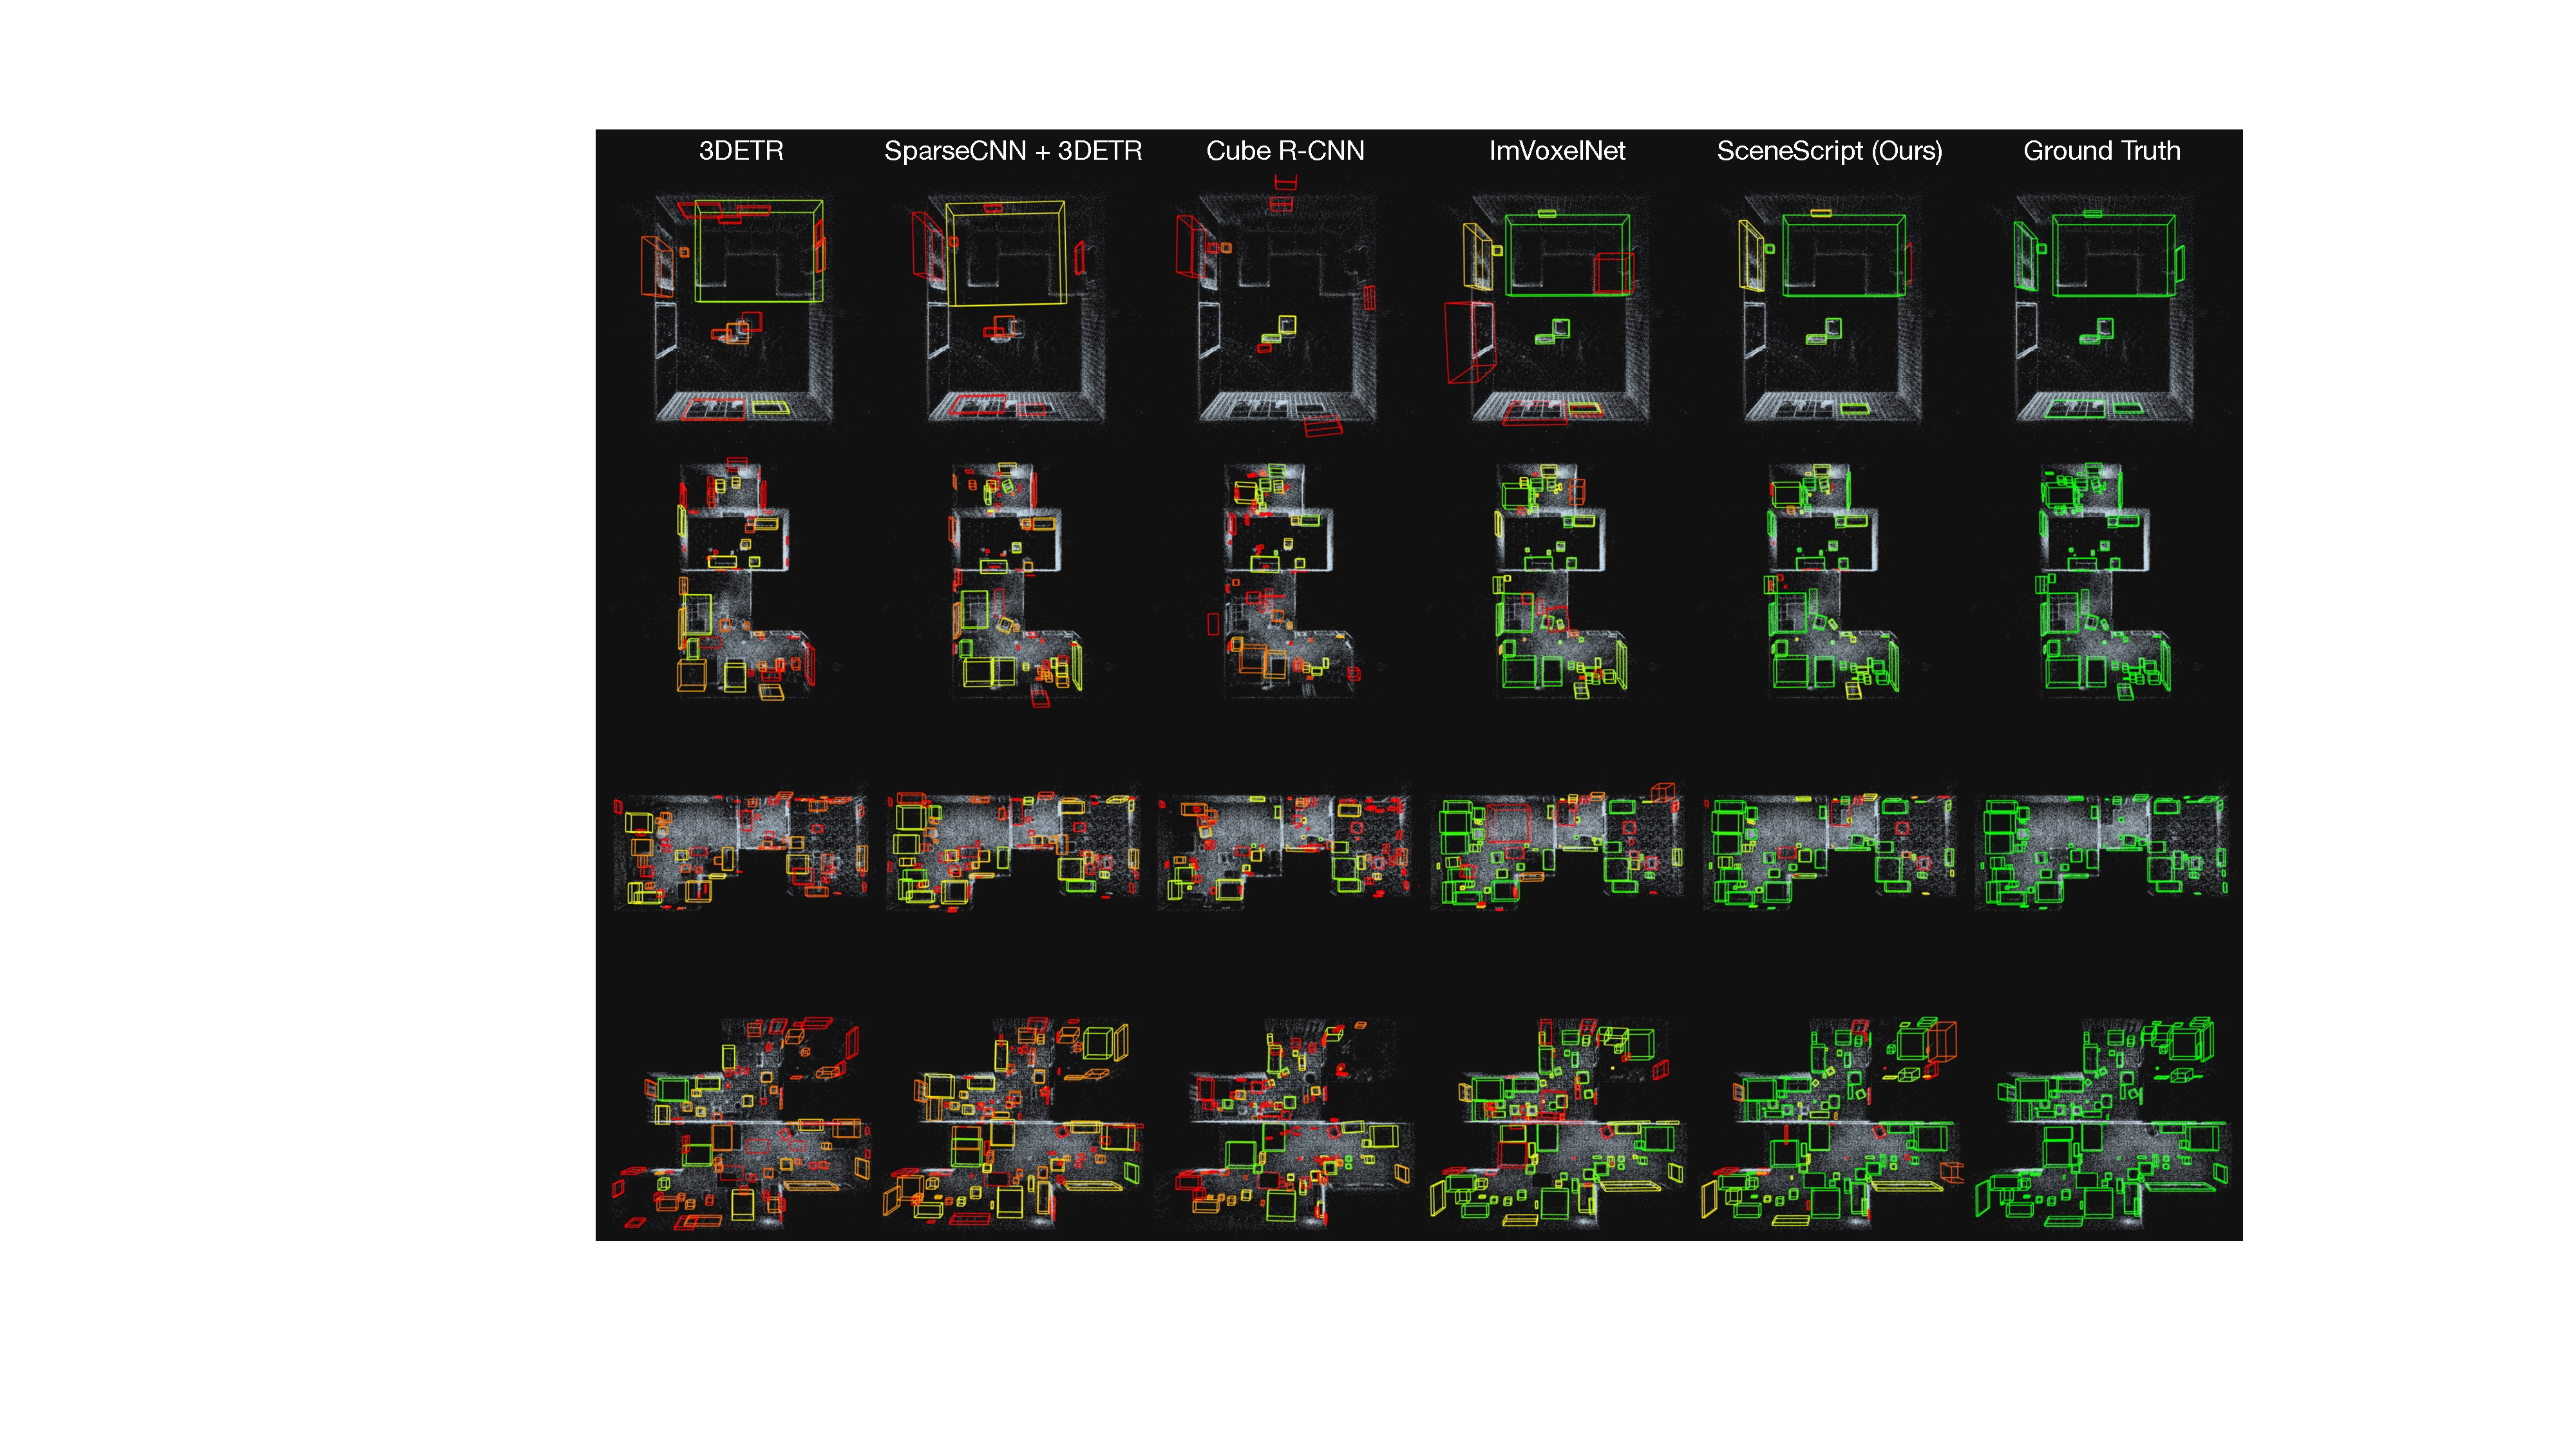
\includegraphics[width=\columnwidth]{figs/ase_bbox_qualitative_iou_compressed.pdf}
    \caption{Qualitative results of predicted bounding boxes on \DatasetName{}. Each bounding box is colored by its IoU with its matched ground truth bounding box. The color is interpolated from green (\textcolor{green}{IoU = 1.0}) to yellow (\textcolor{yellow}{IoU = 0.5}) to red (\textcolor{red}{IoU = 0}).}
    \label{fig:ase_bbox_qualitative_iou}
\end{figure}



\subsection{Qualitative Results on \DatasetName{}}

In Figure~\ref{fig:ase_bbox_qualitative}, we show qualitative results of all the methods trained on \DatasetName{}. This figure demonstrates the difficult of predicting objects in \DatasetName{} as it is very cluttered. Also, due to the generated trajectories not necessarily visiting every part of the scene, some ground truth bounding boxes have very little points associated with them (see the ground truth in row 3. The lower right corner has very few points yet there are bounding boxes present). 

Most methods tend to correctly predict the larger categories (e.g. \textcolor{bed_bbox_color}{bed} and \textcolor{sofa_bbox_color}{sofa}). However, the small object categories (e.g. \textcolor{jar_bbox_color}{jar} and \textcolor{flower_pot_bbox_color}{flower\_pot}) are much harder to detect, thus the ground truth for these categories typically have 0 IoU with predictions (see Figure~\ref{fig:ase_bbox_qualitative_iou} for qualitative predictions visualised with IoU scores). This leads to relatively low F1 scores for some of the baselines (e.g. 3DETR) due to averaging the F1 scores across classes, while visually the predictions look relatively reasonable. We also include results from SparseCNN+3DETR (details can be found in Section~\ref{subsec:sparsecnn_threedetr}). It can be seen from Figures~\ref{fig:ase_bbox_qualitative} and~\ref{fig:ase_bbox_qualitative_iou} that it qualitatively performs better on \DatasetName{} than a pure 3DETR model.




\begin{table}[h]
\centering
    \caption{mAP for baselines trained on \DatasetName.}
    \begin{tabular}{c|c|cc}
        & & \multicolumn{2}{c}{mAP} \\
         Method & Input & @.25 IoU & @.50 IoU \\
        \hline \hline
        3DETR '21~\cite{misra2021end} & Points & 0.148 & 0.040 \\
        SparseCNN~\cite{tang2022torchsparse} + 3DETR~\cite{misra2021end} & Points & 0.308 & 0.115 \\
        Cube R-CNN '23~\cite{brazil2023omni3d} & RGB & 0.383 & 0.181 \\
        ImVoxelNet '22~\cite{rukhovich2022imvoxelnet} & RGB & 0.648 & 0.572\\
    \end{tabular}
    \label{tab:baseline_map}
\end{table}

\subsection{mAP Metrics for Baselines trained on \DatasetName{}}
\label{app:baseline_map}

In Table~\ref{tab:baseline_map}, we list the mAP values for methods trained on \DatasetName{}.



\subsection{Discussion of Average Precision Metric}
Average precision (AP) has become a standard metric for measuring 3D object detection performance. A general outline of the procedure required to calulate this metric is to collect detections across a number of scenes, rank each by descending confidence. Average precision is then computed from this detection pool by framing it as an information retrieval task: order of retrieval determined by the confidence ranking; success of a retrieval determined by an IoU threshold (typically 0.25 or 0.5 for 3D object detection). This framing enables the generation of a precicision-recall curve for the detector, with the average precision given by an approximation of the area underneath this curve.

A drawback of this information retrieval framing is that it is order variant, and requires that the relative certainty of detections across scenes be determinable. While many prior detection methods regress a logit that can naturally represent this certainty, \eg the classification logit is often used, \METHOD{}'s detections are more binary: either the object is present in the predicted sequence or not. Within a single scene, we may be able to leverage a heuristic such as sequence order to determine relative certainty, \ie most certain detections appear sooner in the prediction order (although we have not investigated whether this actually occurs). However, to determine a similar heuristic between scenes would require too many assumptions to be considered a robust and fair evaluation configuration.

\begin{figure}[]
    \centering
    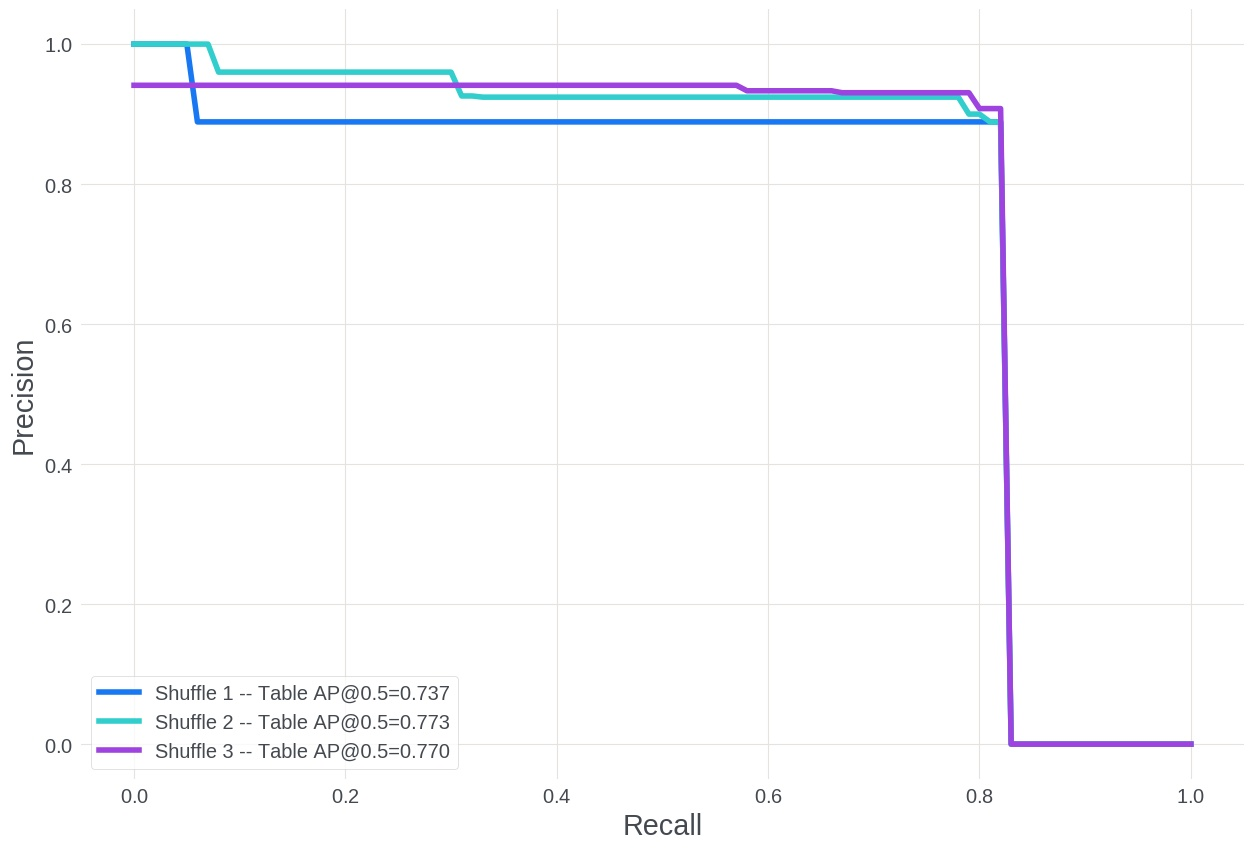
\includegraphics[width=0.5\linewidth]{figs/prec-recall-shuffle.jpg}
    \caption{Precision-recall variance with scene order. The precision-recall curves are plotted for \METHOD{}'s predictions of the \textit{table} class on the same 10 scenes, however the order of those scenes is shuffled for each evaluation. The inability sort predictions across scenes leaves the AP@0.5IoU metric sensitive to the order that scenes are evaluated.}
    \label{fig:prec-rec}
\end{figure}

\begin{table}[]
    \centering
    \caption{Illustration of how average precision is negatively affected by the inability to sort across scenes. Two idential sets of detections are produced by detectors 1 and 2. Detector 1 outputs an absolute measure of confidence allowing for sorting across scenes. However, it is only possible to determine the relative confidence of predictions within a scene for detector 2. This results in a lower AP, as there is no opportunity to rank good predictions from scene B above bad predictions from scene A. We assume there are 3 GT entities in each scene for AP and F1 computation.}
    \begin{tabular}{c| cccccc | cccccc}
     & \multicolumn{6}{c|}{Detector 1} & \multicolumn{6}{c}{Detector 2} \\
     & \multicolumn{6}{c|}{w/ absolute conf.} & \multicolumn{6}{c}{relative conf. only} \\
     \hline \hline
     Scene    & A & B & B & A & B & A & A & A & A & B & B & B \\
     Certainty & high & high & high & med. & low & low     & - & - & - & - & - & - \\
     Success & 1 & 1 & 1 & 0 & 0 & 0    & 1 & 0 & 0 & 1 & 1 & 0 \\
     \hline
     AP & \multicolumn{6}{c|}{0.5} & \multicolumn{6}{c}{0.34} \\
     F1 & \multicolumn{6}{c|}{0.5} & \multicolumn{6}{c}{0.5}
    \end{tabular}
    \label{tab:pr-ranking}
\end{table}

To further illustrate this point, we consider an evaluation setup where we use prediction order within scenes as a proxy for relative certainty, without sorting across scenes. In Figure~\ref{fig:prec-rec} we show precision-recall curves computed over 10 scenes from \DatasetName{} validation set using the assumption. Importantly, each curve on this graph are the \textit{same detections on the same scenes}, but with the scenes simply evaluated in a new, random order each time. Not only is the resulting metric variant with the order of scenes, but low certainty predictions at the end of ascene's predictions may appear earlier in the ranked pool of detections than high certainty predictions from another scene. If these are incorrect, they will arteficially lower the precision achievable, and in turn lower the average precision for a method. A toy example of this is included in Table~\ref{tab:pr-ranking}.

For these reasons, in the main paper we choose to use a F1-score-based metrics to evaluate detection performance. These are not sensitive to ordering as also illustrated in Table~\ref{tab:pr-ranking}.

\begin{figure}[t]
    \centering
    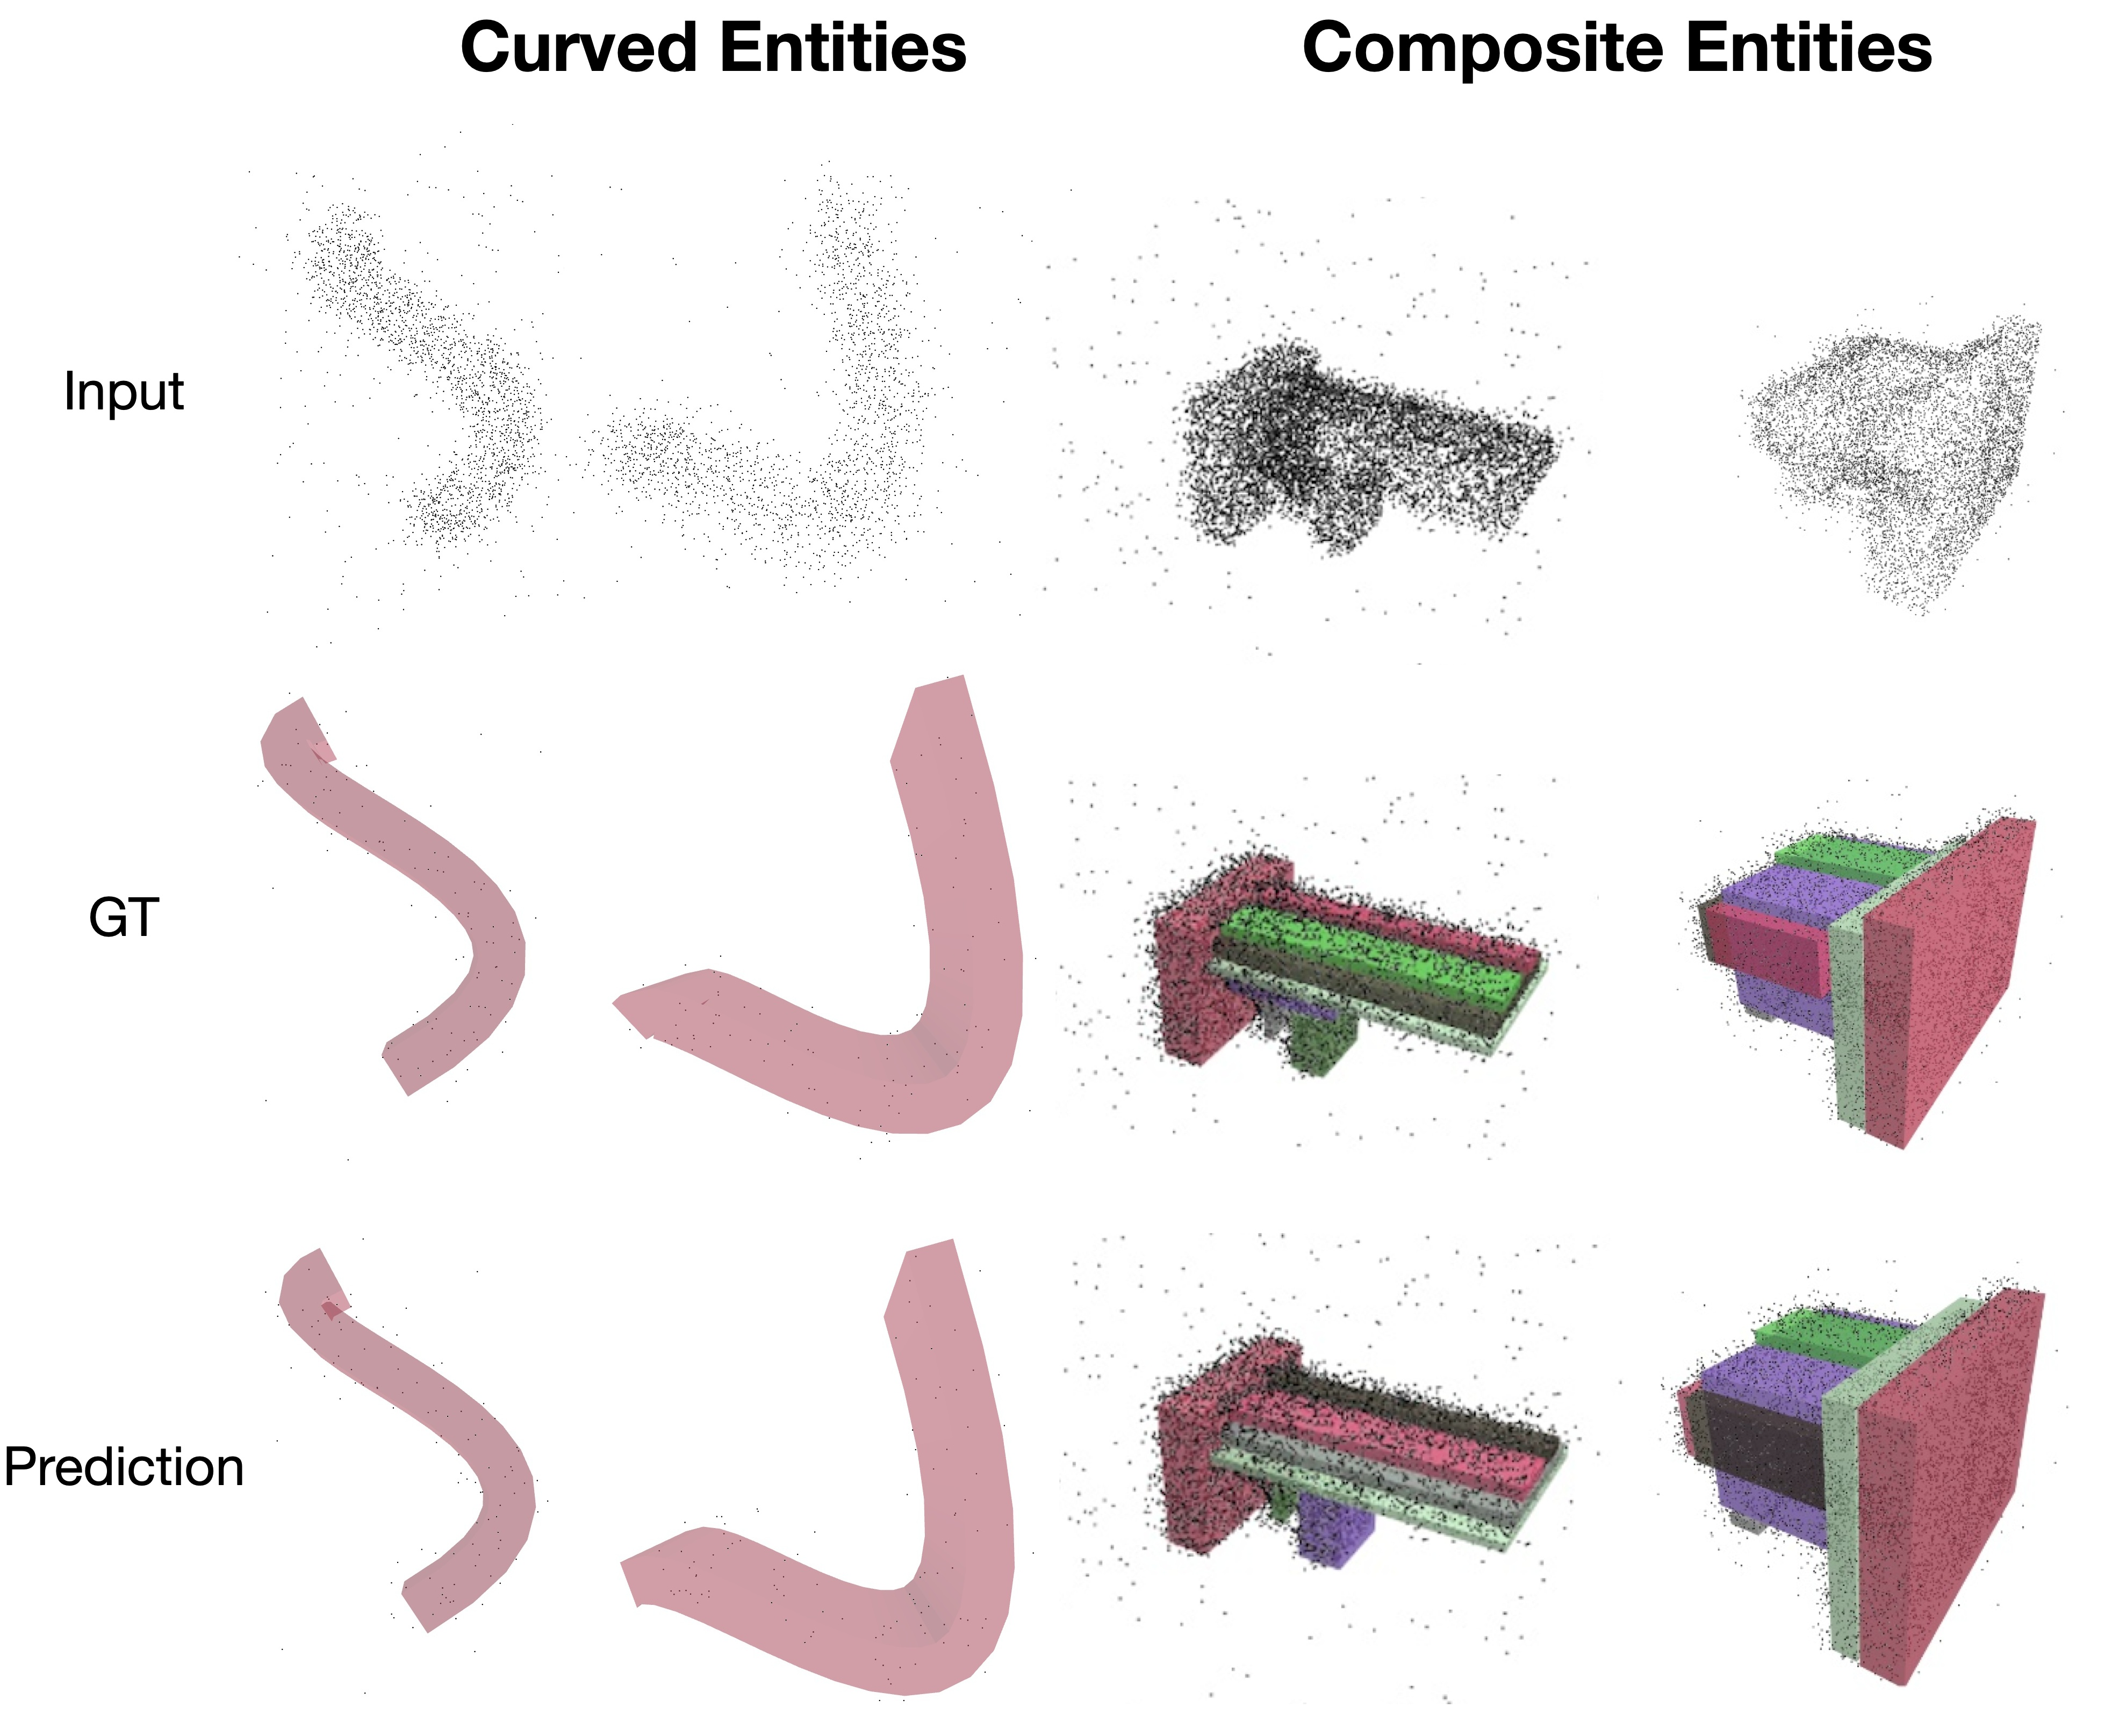
\includegraphics[width=\columnwidth]{figs/fuyang}
    \caption{Non-planar wall geometry extensions to \METHOD. Examples of input point clouds (top row), the prediction 3D shape (middle row),
and ground truth wall shape (bottom row). (left) Examples of Bezier parameterisation for curved walls. (right) Results for wall primitive compositions. We observe that both simple extensions to the parameterisation of the walls can be accurately described and predicted by SceneScript.}
    \label{fig:ext_fuyang}
\end{figure}
\begin{figure}[ht]
    \centering
    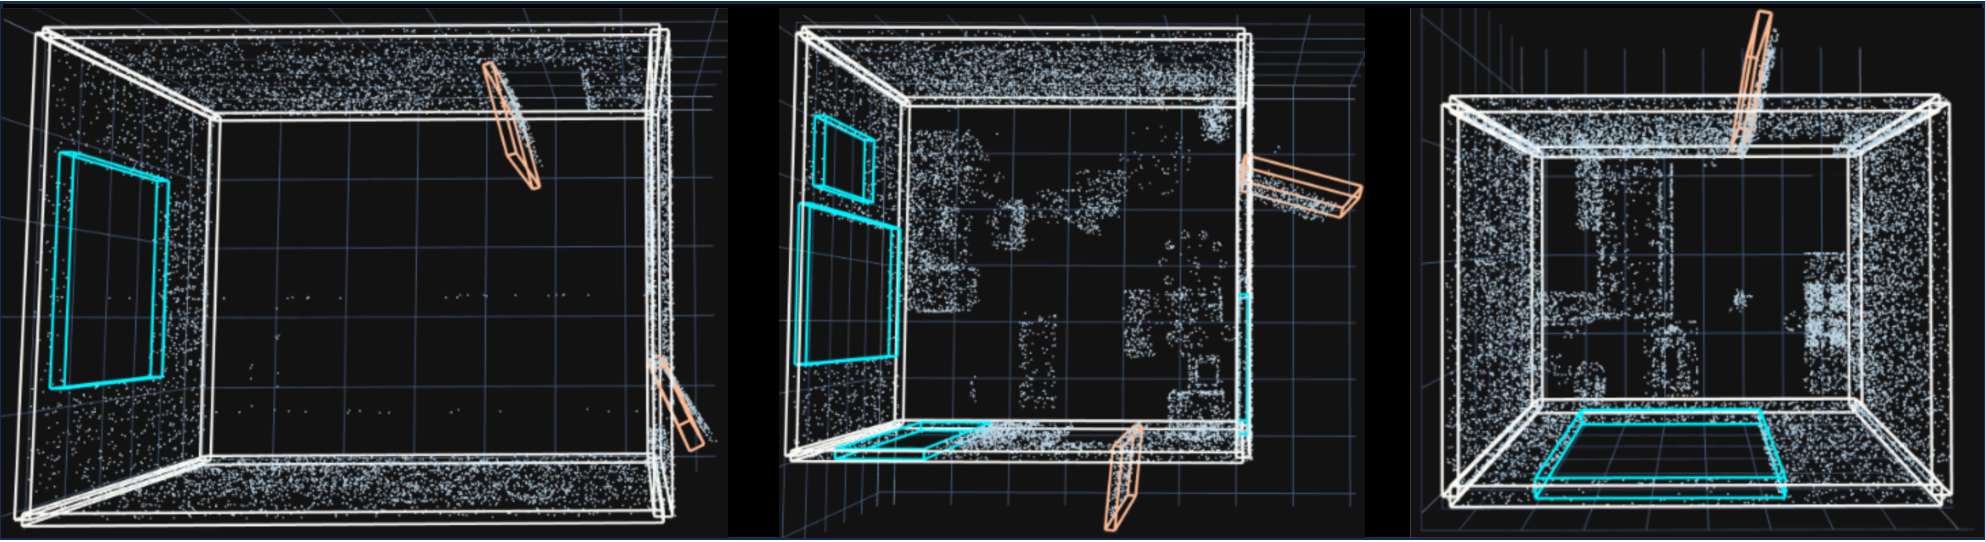
\includegraphics[width=0.9\columnwidth]{figs/door_state.pdf}
    \caption{Results for detecting door state estimation. We visualize the predicted layout on top of the input point cloud.}
    \label{fig:ext_door_state}
\end{figure}

\section{Further Extensions of SceneScript}
\label{app:extensions}
\subsection{Extending \METHOD~with Curved Entities}


In previous layout estimation work, such as \cite{furukawa2009reconstructing,liu2019planercnn},
methods leverage a planar assumption
and use robust estimation procedures custom tailored to planar primitive fitting.
Extending such methods to more complex, non-planar entities is non-trivial and requires significant effort.
In contrast,
we show that our structured language-based approach makes it straightforward to extend to curved walls,
as for example extruded Bezier curves~\cite{beziercurves},
% To do this,
simply by defining a new \texttt{make\_curved\_wall} command. 

The curved wall command is a simple Bezier parametrisation
consisting of 4 additional parameters:
the $x,y$ values of the 2 control points
that define the wall curvature.
Explicitly, our planar wall command changes to: 
\begin{lstlisting}[language=StructuredLanguage]
make_curved_wall: a_x, a_y, a_z, b_x, b_y, b_z, c1_x, c2_y, c2_x, c2_y, height, thickness
\end{lstlisting}
where $c_{1_x}, c_{1_y}, c_{2_x}, c_{2_y}$ are the Bezier control points. 


We generate a synthetic curved walls dataset to train \METHOD.
Example Bezier walls with a qualitative evaluation are in Figure~\ref{fig:ext_fuyang} (left).
The predictions are nearly indistinguishable compared to ground truth,
indicating that our method can learn to predict such complex primitives.

% quantitative evaluation
In a synthetic test bed, we evaluate the capability of our model to infer the control points of walls parameterized on extruded Bezier curves. Quantitative results are shown in Table~\ref{tab:quantitative_eval_bezier_cuves}.

\begin{table}[]
\centering
\caption{Quantitative assessment of the reconstruction of curved walls using extruded Bezier curves as parameters. Token accuracies gauge performance based on a tokenized 1D sequence of the structured language, allowing for a specified slack of +/- N tokens. The IOU is calculated by comparing the interpreted geometry with the GT geometry. We achieve virtually error-free results indicating efficient interplay between parameterization and modelling capability of our method.}
\begin{tabular}{c|c|c}
     Token Acc. Slack 1 & Token Acc. Slack 3 & IOU \\ 
    \hline
       0.993 & 1.0 & 0.990 \\
\end{tabular}
\label{tab:quantitative_eval_bezier_cuves}
\end{table}




\subsection{Extending \METHOD~to Compositions of Wall Primitives}

To demonstrate the extensibility of \METHOD's structured language,
and similarly to the reconstruction of object primitives explored in the main paper, we demonstrate representing complexly shaped walls
as compositions of cuboids.
We define a new parametrization for this class of walls as follows:
\begin{lstlisting}[language=StructuredLanguage]
make_wall: a_x, a_y, ...
make_wall_prim: pos_x, pos_y, pos_z, size_x, size_y, size_z
\end{lstlisting}
where the \texttt{make\_wall\_prim} command describes a cuboid
to be composed with its parent wall entity.
We added such cuboid compositions to a base wall
in Figure~\ref{fig:ext_fuyang} (right).
In this proof-of-concept,
the results of Table~\ref{tab:compositewalls} clearly demonstrate the ability of the network
to infer compositions of cuboids on base walls
only from a noisy surface point cloud.


\begin{table}[]
    \centering
    \caption{Correctly predicted parameters of composite walls as a percentage . Slack $n$ indicates estimation of composite wall parameters within bounds of $n*5cm$.}
    \begin{tabular}{@{}cc||*{3}{c|}}
  \multicolumn{1}{c}{}  &   &\multicolumn{3}{|c|}{Occlusion Levels}\\
    \multicolumn{1}{c}{} & & No    & Light    &High       \\ \hline \hline
    \multirow{3}*{\rotatebox{90}{Slack}}  
   & 1 & 99.6 & 95.9   & 92.6    \\ 
   & 3 & 99.9    &96.4 & 93.3     \\ 
   & 5 & 100    & 98.2    & 95.5   \\ 
   \end{tabular}
    \label{tab:compositewalls}
\end{table}
  
\subsection{Extending \METHOD~to Object States}

% To illustrate the flexibility of our method, we showcase how trivially we can add entity state estimation to our pipeline. 
Yet another simple extension to our \METHOD~language allows us to represent door states, w.r.t their opening configuration. For this, we simply change the original door representation to include a list of parameters that define door state as follows:


\begin{figure}[t]
    \centering
    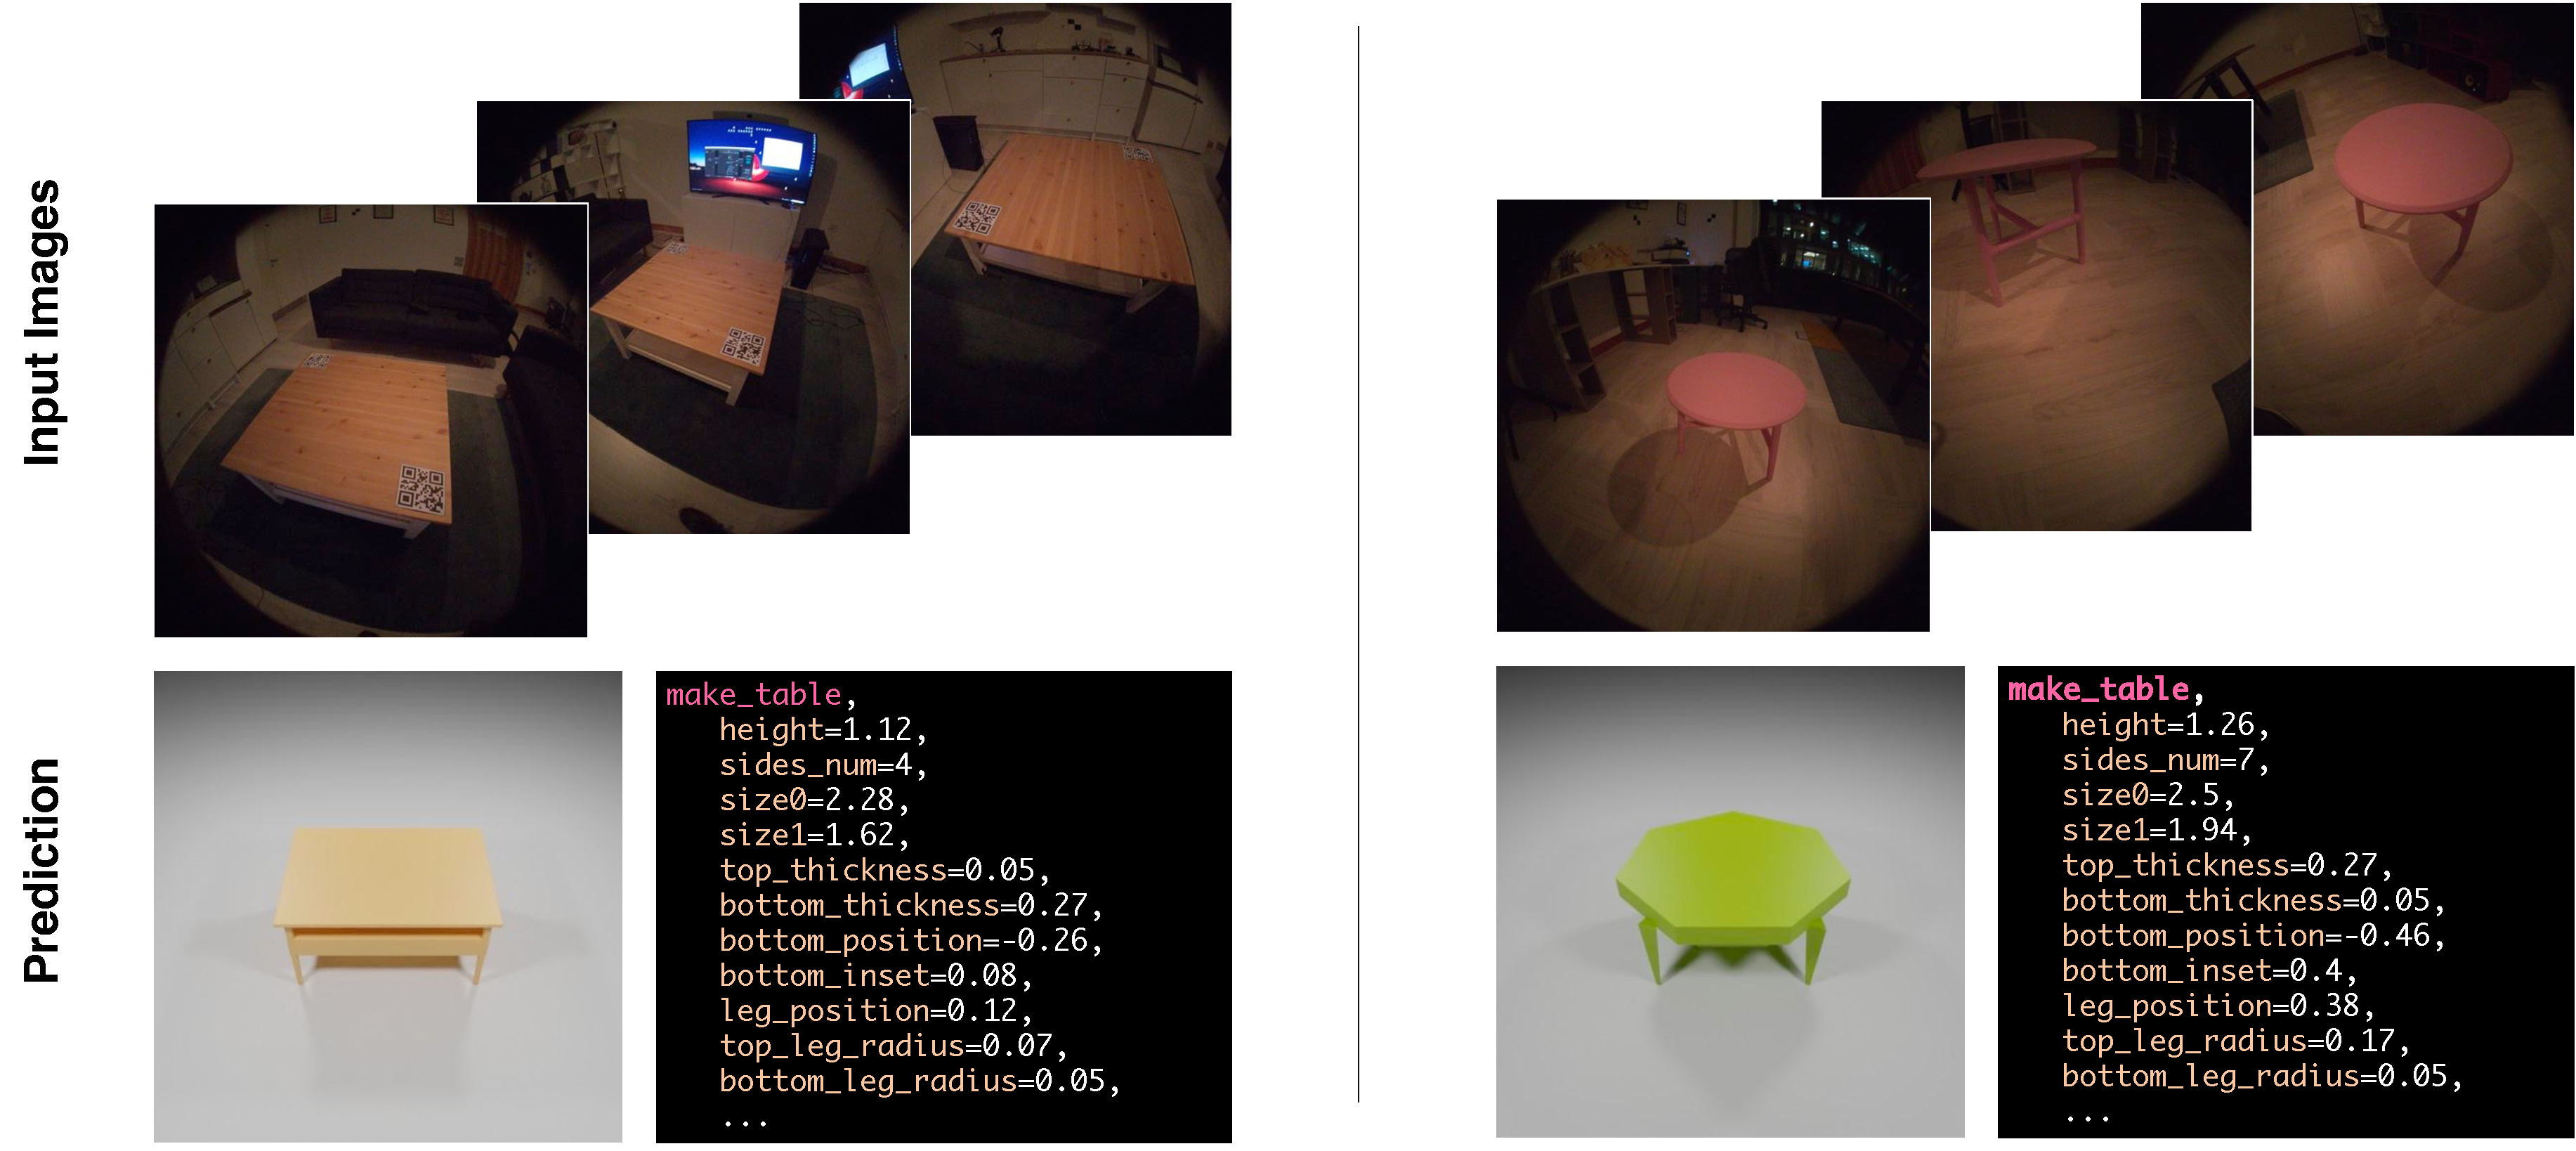
\includegraphics[width=\columnwidth]{figs/blender_horiz.pdf}
    \caption{Two real-world inferences based on a Blender Geometry Node [3] obtained online. Input RGB images are recorded on an Aria device. We visualize a subset of the predicted language as well as the geometry obtained by inputting that prediction into the Geometry Node.}
    \label{fig:ext_blender}
\end{figure}


\begin{lstlisting}[language=StructuredLanguage]
make_door: id, wall_id, pos_x, pos_y, pos_z, width, height, open_degree, hinge_side, open_direction
\end{lstlisting}
\texttt{hinge\_side} represents which side of the door the hinge is on, \texttt{open\_direction} determines whether the door opens into the room or outside of the room, and \texttt{open\_degree} is the angle of the opening.
In Figure~\ref{fig:ext_door_state} (second),
we qualitatively demonstrate object state estimation.
We annotated our doors
with a new command parameterisation
extended by door hinge position, wall opening side and opening angle.
As with our other extensions,
our model is able to handle this situation without issue.
This small GT language extension demonstrates effective state estimation
while the input and network architecture remain unchanged.

\subsection{Extending \METHOD~to Blender Parametric Object Models}

Parametric modelling offers detailed high-quality geometry representations along with interpretability and editability by design~\cite{jones2020shapeassembly,jones2021shapemod,jones2022plad,pearl2022geocode}. 
The Blender community offers readily accessible Geometry Nodes of diverse object categories as a procedural language.
We investigate the use of a particular Geometry Node for tables~\cite{mrBash2023Tables}.
% shown in Figure~\ref{fig:extensions} (right center).
Not only can we directly incorporate this parametric model
into our \METHOD~language,
but we can also use it to generate data
by randomly sampling its parameters
similar to~\cite{pearl2022geocode}. 

We design a simple proof-of-concept experiment where we render synthetic RGB images of random tables, composite them on a random image background, and learn to predict the ground truth Blender procedural language.
In Figure~\ref{fig:ext_blender}, we demonstrate two real-world inferences of tables using this language, showing our method is capable of predicting reasonable parameters to reconstruct these tables. Interestingly, in the second example the model predicts a high \texttt{sides\_num} to approximate the circular tabletop, which was not on the training set.

% ---- Bibliography ----
%
% BibTeX users should specify bibliography style 'splncs04'.
% References will then be sorted and formatted in the correct style.
%
\bibliographystyle{splncs04}
\bibliography{main}

% \clearpage
% supp mat

\end{document}
